%%========================================================================
%% LaTeX sjabloon voor stage/projectrapport of bachelorproef
%%  HoGent Bedrijf en Organisatie
%%========================================================================

\documentclass[12pt, fleqn, a4paper]{book}

%%---------- Documenteigenschappen ---------------------------------------
%% Vul dit aan met je eigen info:

% Je eigen naam
\newcommand{\student}{Michiel De Wilde}

% De naam van je lector, begeleider, promotor
\newcommand{\promotor}{Antonia Pierreux}

% De naam van je co-promotor
\newcommand{\copromotor}{Philippe De Wilde}

% Indien je bachelorproef in opdracht van een bedrijf of organisatie
% geschreven is, geef je hier de naam.
\newcommand{\instelling}{Hogeschool Gent}

% De titel van het rapport/bachelorproef
\newcommand{\titel}{Use Cases voor Unikernels}

% Datum van indienen
\newcommand{\datum}{9 januari 2017}

% Faculteit
\newcommand{\faculteit}{Faculteit Bedrijf en Organisatie}

% Soort rapport
\newcommand{\rapporttype}{Scriptie voorgedragen tot het bekomen van de graad van\\Bachelor in de toegepaste informatica}

% Academiejaar
\newcommand{\academiejaar}{2016-2017}

% Examenperiode
%  - 1e semester = 1e examenperiode
%  - 2e semester = 2e examenperiode
%  - tweede zit = 3e examenperiode
\newcommand{\examenperiode}{1e examenperiode}


\usepackage[top=3cm,bottom=3cm,left=3cm,right=3cm,headsep=10pt,a4paper]{geometry} % Page margins
\usepackage[utf8]{inputenc}  % Accenten gebruiken in tekst (vb. é ipv \'e)
\usepackage{amsfonts}        % AMS math packages: extra wiskundige
\usepackage{amsmath}         %   symbolen (o.a. getallen-
\usepackage{amssymb}         %   verzamelingen N, R, Z, Q, etc.)
\usepackage[dutch,american]{babel}    % Taalinstellingen: woordsplitsingen,
                             %  commando's voor speciale karakters
                             %  ("dutch" voor NL)
\usepackage{iflang}
\usepackage{eurosym}         % Euro-symbool €
\usepackage{geometry}
\usepackage{graphicx}        % Invoegen van tekeningen
\graphicspath{{img/}}
\usepackage{tikz}            % Required for drawing custom shapes
\usepackage[pdftex,bookmarks=true]{hyperref}
\usepackage{wrapfig}         % Positioneren van tekeningen
\usepackage[pdftex,bookmarks=true]{hyperref}
                             % PDF krijgt klikbare links & verwijzingen,
                             %  inhoudstafel
\usepackage{listings}        % Broncode mooi opmaken
\usepackage{multirow}        % Tekst over verschillende cellen in tabellen
\usepackage{rotating}        % Tabellen en figuren roteren
\usepackage{fancyhdr}        % Pagina-opmaak met hoofd- en voettekst

\usepackage[T1]{fontenc}     % Ivm lettertypes
\usepackage{lmodern}
\usepackage{textcomp}
\usepackage{listingsutf8}

\usepackage{booktabs}        % Required for nicer horizontal rules in tables

\usepackage{xcolor}          % Required for specifying colors by name
\definecolor{maincolor}{RGB}{0,147,208} % Define the main color used for 
                             % highlighting throughout the book
                             % 0, 147, 208 = officiële kleur HoGent FBO

% Paragraph style: no indent, add space between paragraphs
\setlength{\parindent}{0em}
\setlength{\parskip}{1em}

\usepackage{etoolbox}
\usepackage{titling} % Macros for title, author, etc
\usepackage[toc,page]{appendix}
\usepackage{pdfpages}

%----------------------------------------------------------------------------------------
%	FONTS
%----------------------------------------------------------------------------------------

\usepackage{avant} % Use the Avantgarde font for headings
%\usepackage{times} % Use the Times font for headings
\usepackage{mathptmx} % Use the Adobe Times Roman as the default text font together with math symbols from the Sym­bol, Chancery and Com­puter Modern fonts

\usepackage{microtype} % Slightly tweak font spacing for aesthetics
\usepackage[utf8]{inputenc} % Required for including letters with accents
\usepackage[T1]{fontenc} % Use 8-bit encoding that has 256 glyphs

%----------------------------------------------------------------------------------------
% BIBLIOGRAPHY AND INDEX
%----------------------------------------------------------------------------------------

\usepackage{csquotes}
\usepackage[style=apa,backend=biber,url=false,doi=false]{biblatex}
\DeclareLanguageMapping{american}{american-apa}
\addbibresource{tin-bachproef.bib} % BibTeX bibliography file
\defbibheading{bibempty}{}

\usepackage{calc} % For simpler calculation - used for spacing the index letter headings correctly
\usepackage{makeidx} % Required to make an index
\makeindex % Tells LaTeX to create the files required for indexing

%%---------- Layout ------------------------------------------------------

% hoofdingen, enz.
\pagestyle{fancy}
% enkel hoofdstuktitel in hoofding, geen sectietitel (vermijd overlap)
\renewcommand{\sectionmark}[1]{}

% lijn, wordt gebruikt in titelpagina
\newcommand{\HRule}{\rule{\linewidth}{0.5mm}}

% Leeg blad
\newcommand{\emptypage}{
\newpage
\thispagestyle{empty}
\mbox{}
\newpage
}

% Gebruik een schreefloos lettertype ipv het "oubollig" uitziende
% Computer Modern
\renewcommand{\familydefault}{\sfdefault}

%------------------------------------------------------------------------------
%	TITLE PAGE
%------------------------------------------------------------------------------

\newcommand{\inserttitlepage}{%
\begin{titlepage}
  \newgeometry{top=2cm,bottom=1.5cm,left=1.5cm,right=1.5cm}
  \begin{center}

    \begingroup
    \rmfamily
    
\includegraphics[width=2.5cm]{img/HG-beeldmerk-woordmerk}\\[.5cm]
    Faculteit Bedrijf en Organisatie\\[3cm]
    \titel
    \vfill
    \student\\[3.5cm]
    Scriptie voorgedragen tot het bekomen van de graad van\\professionele bachelor in de toegepaste informatica\\[2cm]
    Promotor:\\
    \promotor\\
    \ifdefempty{\copromotor}{\vspace{2.5cm}}{Co-promotor:\\\copromotor\\[2.5cm]}
    Instelling: \instelling\\[.5cm]
    Academiejaar: \academiejaar\\[.5cm]
    \ifcase \examenperiode \or Eerste \or Tweede \else Derde \fi examenperiode
    \endgroup

  \end{center}
  \restoregeometry
\end{titlepage}
  \emptypage
\begin{titlepage}
  \newgeometry{top=5.35cm,bottom=1.5cm,left=1.5cm,right=1.5cm}
  \begin{center}

    \begingroup
    \rmfamily
    \IfLanguageName{dutch}{Faculteit Bedrijf en Organisatie}{Faculty of Business and Information Management}\\[3cm]
    \titel
    \vfill
    \student\\[3.5cm]
    \IfLanguageName{dutch}{Scriptie voorgedragen tot het bekomen van de graad van\\professionele bachelor in de toegepaste informatica}{Thesis submitted in partial fulfillment of the requirements for the degree of\\professional bachelor of applied computer science}\\[2cm]
    Promotor:\\
    \promotor\\
    \ifdefempty{\copromotor}{\vspace{2.5cm}}{Co-promotor:\\\copromotor\\[2.5cm]}
    \IfLanguageName{dutch}{Instelling}{Institution}: \instelling\\[.5cm]
    \IfLanguageName{dutch}{Academiejaar}{Academic year}: \academiejaar\\[.5cm]
    \IfLanguageName{dutch}{%
    \ifcase \examenperiode \or Eerste \or Tweede \else Derde \fi examenperiode}{%
    \ifcase \examenperiode \or First \or Second \else Third \fi examination period}
    \endgroup

  \end{center}
  \restoregeometry
\end{titlepage}
}

%----------------------------------------------------------------------------------------
%	MAIN TABLE OF CONTENTS
%----------------------------------------------------------------------------------------

\usepackage{titletoc} % Required for manipulating the table of contents

\contentsmargin{0cm} % Removes the default margin

% Part text styling
\titlecontents{part}[0cm]
{\addvspace{20pt}\centering\large\bfseries}
{}
{}
{}

% Chapter text styling
\titlecontents{chapter}[1.25cm] % Indentation
{\addvspace{12pt}\large\sffamily\bfseries} % Spacing and font options for chapters
{\color{maincolor!60}\contentslabel[\Large\thecontentslabel]{1.25cm}\color{maincolor}} % Chapter number
{\color{maincolor}}
{\color{maincolor!60}\normalsize\;\titlerule*[.5pc]{.}\;\thecontentspage} % Page number

% Section text styling
\titlecontents{section}[1.25cm] % Indentation
{\addvspace{3pt}\sffamily\bfseries} % Spacing and font options for sections
{\contentslabel[\thecontentslabel]{1.25cm}} % Section number
{}
{\hfill\color{black}\thecontentspage} % Page number
[]

% Subsection text styling
\titlecontents{subsection}[1.25cm] % Indentation
{\addvspace{1pt}\sffamily\small} % Spacing and font options for subsections
{\contentslabel[\thecontentslabel]{1.25cm}} % Subsection number
{}
{\ \titlerule*[.5pc]{.}\;\thecontentspage} % Page number
[]

% List of figures
\titlecontents{figure}[0em]
{\addvspace{-5pt}\sffamily}
{\thecontentslabel\hspace*{1em}}
{}
{\ \titlerule*[.5pc]{.}\;\thecontentspage}
[]

% List of tables
\titlecontents{table}[0em]
{\addvspace{-5pt}\sffamily}
{\thecontentslabel\hspace*{1em}}
{}
{\ \titlerule*[.5pc]{.}\;\thecontentspage}
[]

%----------------------------------------------------------------------------------------
%	MINI TABLE OF CONTENTS IN PART HEADS
%----------------------------------------------------------------------------------------

% Chapter text styling
\titlecontents{lchapter}[0em] % Indenting
{\addvspace{15pt}\large\sffamily\bfseries} % Spacing and font options for chapters
{\color{maincolor}\contentslabel[\Large\thecontentslabel]{1.25cm}\color{maincolor}} % Chapter number
{}
{\color{maincolor}\normalsize\sffamily\bfseries\;\titlerule*[.5pc]{.}\;\thecontentspage} % Page number

% Section text styling
\titlecontents{lsection}[0em] % Indenting
{\sffamily\small} % Spacing and font options for sections
{\contentslabel[\thecontentslabel]{1.25cm}} % Section number
{}
{}

% Subsection text styling
\titlecontents{lsubsection}[.5em] % Indentation
{\normalfont\footnotesize\sffamily} % Font settings
{}
{}
{}

%----------------------------------------------------------------------------------------
%	PAGE HEADERS
%----------------------------------------------------------------------------------------

\usepackage{fancyhdr} % Required for header and footer configuration

\pagestyle{fancy}
\renewcommand{\chaptermark}[1]{\markboth{\sffamily\normalsize\bfseries\chaptername\ \thechapter.\ #1}{}} % Chapter text font settings
\renewcommand{\sectionmark}[1]{\markright{\sffamily\normalsize\thesection\hspace{5pt}#1}{}} % Section text font settings
\fancyhf{} \fancyhead[LE,RO]{\sffamily\normalsize\thepage} % Font setting for the page number in the header
\fancyhead[LO]{\rightmark} % Print the nearest section name on the left side of odd pages
\fancyhead[RE]{\leftmark} % Print the current chapter name on the right side of even pages
\renewcommand{\headrulewidth}{0.5pt} % Width of the rule under the header
\addtolength{\headheight}{2.5pt} % Increase the spacing around the header slightly
\renewcommand{\footrulewidth}{0pt} % Removes the rule in the footer
\fancypagestyle{plain}{\fancyhead{}\renewcommand{\headrulewidth}{0pt}} % Style for when a plain pagestyle is specified

% Removes the header from odd empty pages at the end of chapters
\makeatletter
\renewcommand{\cleardoublepage}{
\clearpage\ifodd\c@page\else
\hbox{}
\vspace*{\fill}
\thispagestyle{empty}
\newpage
\fi}

%----------------------------------------------------------------------------------------
%	THEOREM STYLES
%----------------------------------------------------------------------------------------

\usepackage{amsmath,amsfonts,amssymb,amsthm} % For math equations, theorems, symbols, etc

\newcommand{\intoo}[2]{\mathopen{]}#1\,;#2\mathclose{[}}
\newcommand{\ud}{\mathop{\mathrm{{}d}}\mathopen{}}
\newcommand{\intff}[2]{\mathopen{[}#1\,;#2\mathclose{]}}
\newtheorem{notation}{Notation}[chapter]

% Boxed/framed environments
\newtheoremstyle{maincolornumbox}% % Theorem style name
{0pt}% Space above
{0pt}% Space below
{\normalfont}% % Body font
{}% Indent amount
{\small\bf\sffamily\color{maincolor}}% % Theorem head font
{\;}% Punctuation after theorem head
{0.25em}% Space after theorem head
{\small\sffamily\color{maincolor}\thmname{#1}\nobreakspace\thmnumber{\@ifnotempty{#1}{}\@upn{#2}}% Theorem text (e.g. Theorem 2.1)
\thmnote{\nobreakspace\the\thm@notefont\sffamily\bfseries\color{black}---\nobreakspace#3.}} % Optional theorem note
\renewcommand{\qedsymbol}{$\blacksquare$}% Optional qed square

\newtheoremstyle{blacknumex}% Theorem style name
{5pt}% Space above
{5pt}% Space below
{\normalfont}% Body font
{} % Indent amount
{\small\bf\sffamily}% Theorem head font
{\;}% Punctuation after theorem head
{0.25em}% Space after theorem head
{\small\sffamily{\tiny\ensuremath{\blacksquare}}\nobreakspace\thmname{#1}\nobreakspace\thmnumber{\@ifnotempty{#1}{}\@upn{#2}}% Theorem text (e.g. Theorem 2.1)
\thmnote{\nobreakspace\the\thm@notefont\sffamily\bfseries---\nobreakspace#3.}}% Optional theorem note

\newtheoremstyle{blacknumbox} % Theorem style name
{0pt}% Space above
{0pt}% Space below
{\normalfont}% Body font
{}% Indent amount
{\small\bf\sffamily}% Theorem head font
{\;}% Punctuation after theorem head
{0.25em}% Space after theorem head
{\small\sffamily\thmname{#1}\nobreakspace\thmnumber{\@ifnotempty{#1}{}\@upn{#2}}% Theorem text (e.g. Theorem 2.1)
\thmnote{\nobreakspace\the\thm@notefont\sffamily\bfseries---\nobreakspace#3.}}% Optional theorem note

% Non-boxed/non-framed environments
\newtheoremstyle{maincolornum}% % Theorem style name
{5pt}% Space above
{5pt}% Space below
{\normalfont}% % Body font
{}% Indent amount
{\small\bf\sffamily\color{maincolor}}% % Theorem head font
{\;}% Punctuation after theorem head
{0.25em}% Space after theorem head
{\small\sffamily\color{maincolor}\thmname{#1}\nobreakspace\thmnumber{\@ifnotempty{#1}{}\@upn{#2}}% Theorem text (e.g. Theorem 2.1)
\thmnote{\nobreakspace\the\thm@notefont\sffamily\bfseries\color{black}---\nobreakspace#3.}} % Optional theorem note
\renewcommand{\qedsymbol}{$\blacksquare$}% Optional qed square
\makeatother

% Defines the theorem text style for each type of theorem to one of the three styles above
\newcounter{dummy}
\numberwithin{dummy}{section}
\theoremstyle{maincolornumbox}
\newtheorem{theoremeT}[dummy]{Theorem}
\newtheorem{problem}{Problem}[chapter]
\newtheorem{exerciseT}{Exercise}[chapter]
\theoremstyle{blacknumex}
\newtheorem{exampleT}{Example}[chapter]
\theoremstyle{blacknumbox}
\newtheorem{vocabulary}{Vocabulary}[chapter]
\newtheorem{definitionT}{Definition}[section]
\newtheorem{corollaryT}[dummy]{Corollary}
\theoremstyle{maincolornum}
\newtheorem{proposition}[dummy]{Proposition}

%----------------------------------------------------------------------------------------
%	DEFINITION OF COLORED BOXES
%----------------------------------------------------------------------------------------

\RequirePackage[framemethod=default]{mdframed} % Required for creating the theorem, definition, exercise and corollary boxes

% Theorem box
\newmdenv[skipabove=7pt,
skipbelow=7pt,
backgroundcolor=black!5,
linecolor=maincolor,
innerleftmargin=5pt,
innerrightmargin=5pt,
innertopmargin=5pt,
leftmargin=0cm,
rightmargin=0cm,
innerbottommargin=5pt]{tBox}

% Exercise box
\newmdenv[skipabove=7pt,
skipbelow=7pt,
rightline=false,
leftline=true,
topline=false,
bottomline=false,
backgroundcolor=maincolor!10,
linecolor=maincolor,
innerleftmargin=5pt,
innerrightmargin=5pt,
innertopmargin=5pt,
innerbottommargin=5pt,
leftmargin=0cm,
rightmargin=0cm,
linewidth=4pt]{eBox}

% Definition box
\newmdenv[skipabove=7pt,
skipbelow=7pt,
rightline=false,
leftline=true,
topline=false,
bottomline=false,
linecolor=maincolor,
innerleftmargin=5pt,
innerrightmargin=5pt,
innertopmargin=0pt,
leftmargin=0cm,
rightmargin=0cm,
linewidth=4pt,
innerbottommargin=0pt]{dBox}

% Corollary box
\newmdenv[skipabove=7pt,
skipbelow=7pt,
rightline=false,
leftline=true,
topline=false,
bottomline=false,
linecolor=gray,
backgroundcolor=black!5,
innerleftmargin=5pt,
innerrightmargin=5pt,
innertopmargin=5pt,
leftmargin=0cm,
rightmargin=0cm,
linewidth=4pt,
innerbottommargin=5pt]{cBox}

% Creates an environment for each type of theorem and assigns it a theorem text style from the "Theorem Styles" section above and a colored box from above
\newenvironment{theorem}{\begin{tBox}\begin{theoremeT}}{\end{theoremeT}\end{tBox}}
\newenvironment{exercise}{\begin{eBox}\begin{exerciseT}}{\hfill{\color{maincolor}\tiny\ensuremath{\blacksquare}}\end{exerciseT}\end{eBox}}
\newenvironment{definition}{\begin{dBox}\begin{definitionT}}{\end{definitionT}\end{dBox}}
\newenvironment{example}{\begin{exampleT}}{\hfill{\tiny\ensuremath{\blacksquare}}\end{exampleT}}
\newenvironment{corollary}{\begin{cBox}\begin{corollaryT}}{\end{corollaryT}\end{cBox}}

%----------------------------------------------------------------------------------------
%	REMARK ENVIRONMENT
%----------------------------------------------------------------------------------------

\newenvironment{remark}{\par\vspace{10pt}\small % Vertical white space above the remark and smaller font size
\begin{list}{}{
\leftmargin=35pt % Indentation on the left
\rightmargin=25pt}\item\ignorespaces % Indentation on the right
\makebox[-2.5pt]{\begin{tikzpicture}[overlay]
\node[draw=maincolor!60,line width=1pt,circle,fill=maincolor!25,font=\sffamily\bfseries,inner sep=2pt,outer sep=0pt] at (-15pt,0pt){\textcolor{maincolor}{R}};\end{tikzpicture}} % Orange R in a circle
\advance\baselineskip -1pt}{\end{list}\vskip5pt} % Tighter line spacing and white space after remark

%----------------------------------------------------------------------------------------
%	SECTION NUMBERING IN THE MARGIN
%----------------------------------------------------------------------------------------

\makeatletter
\renewcommand{\@seccntformat}[1]{\llap{\textcolor{maincolor}{\csname the#1\endcsname}\hspace{1em}}}
\renewcommand{\section}{\@startsection{section}{1}{\z@}
{-4ex \@plus -1ex \@minus -.4ex}
{1ex \@plus.2ex }
{\normalfont\large\sffamily\bfseries}}
\renewcommand{\subsection}{\@startsection {subsection}{2}{\z@}
{-3ex \@plus -0.1ex \@minus -.4ex}
{0.5ex \@plus.2ex }
{\normalfont\sffamily\bfseries}}
\renewcommand{\subsubsection}{\@startsection {subsubsection}{3}{\z@}
{-2ex \@plus -0.1ex \@minus -.2ex}
{.2ex \@plus.2ex }
{\normalfont\small\sffamily\bfseries}}
\renewcommand\paragraph{\@startsection{paragraph}{4}{\z@}
{-2ex \@plus-.2ex \@minus .2ex}
{.1ex}
{\normalfont\small\sffamily\bfseries}}

%----------------------------------------------------------------------------------------
%	PART HEADINGS
%----------------------------------------------------------------------------------------

% numbered part in the table of contents
\newcommand{\@mypartnumtocformat}[2]{%
\setlength\fboxsep{0pt}%
\noindent\colorbox{maincolor!20}{\strut\parbox[c][.7cm]{\ecart}{\color{maincolor!70}\Large\sffamily\bfseries\centering#1}}\hskip\esp\colorbox{maincolor!40}{\strut\parbox[c][.7cm]{\linewidth-\ecart-\esp}{\Large\sffamily\centering#2}}}%
%%%%%%%%%%%%%%%%%%%%%%%%%%%%%%%%%%
% unnumbered part in the table of contents
\newcommand{\@myparttocformat}[1]{%
\setlength\fboxsep{0pt}%
\noindent\colorbox{maincolor!40}{\strut\parbox[c][.7cm]{\linewidth}{\Large\sffamily\centering#1}}}%
%%%%%%%%%%%%%%%%%%%%%%%%%%%%%%%%%%
\newlength\esp
\setlength\esp{4pt}
\newlength\ecart
\setlength\ecart{1.2cm-\esp}
\newcommand{\thepartimage}{}%
\newcommand{\partimage}[1]{\renewcommand{\thepartimage}{#1}}%
\def\@part[#1]#2{%
\ifnum \c@secnumdepth >-2\relax%
\refstepcounter{part}%
\addcontentsline{toc}{part}{\texorpdfstring{\protect\@mypartnumtocformat{\thepart}{#1}}{\partname~\thepart\ ---\ #1}}
\else%
\addcontentsline{toc}{part}{\texorpdfstring{\protect\@myparttocformat{#1}}{#1}}%
\fi%
\startcontents%
\markboth{}{}%
{\thispagestyle{empty}%
\begin{tikzpicture}[remember picture,overlay]%
\node at (current page.north west){\begin{tikzpicture}[remember picture,overlay]%
\fill[maincolor!20](0cm,0cm) rectangle (\paperwidth,-\paperheight);
\node[anchor=north] at (4cm,-3.25cm){\color{maincolor!40}\fontsize{220}{100}\sffamily\bfseries\@Roman\c@part};
\node[anchor=south east] at (\paperwidth-1cm,-\paperheight+1cm){\parbox[t][][t]{8.5cm}{
\printcontents{l}{0}{\setcounter{tocdepth}{1}}%
}};
\node[anchor=north east] at (\paperwidth-1.5cm,-3.25cm){\parbox[t][][t]{15cm}{\strut\raggedleft\color{white}\fontsize{30}{30}\sffamily\bfseries#2}};
\end{tikzpicture}};
\end{tikzpicture}}%
\@endpart}
\def\@spart#1{%
\startcontents%
\phantomsection
{\thispagestyle{empty}%
\begin{tikzpicture}[remember picture,overlay]%
\node at (current page.north west){\begin{tikzpicture}[remember picture,overlay]%
\fill[maincolor!20](0cm,0cm) rectangle (\paperwidth,-\paperheight);
\node[anchor=north east] at (\paperwidth-1.5cm,-3.25cm){\parbox[t][][t]{15cm}{\strut\raggedleft\color{white}\fontsize{30}{30}\sffamily\bfseries#1}};
\end{tikzpicture}};
\end{tikzpicture}}
\addcontentsline{toc}{part}{\texorpdfstring{%
\setlength\fboxsep{0pt}%
\noindent\protect\colorbox{maincolor!40}{\strut\protect\parbox[c][.7cm]{\linewidth}{\Large\sffamily\protect\centering #1\quad\mbox{}}}}{#1}}%
\@endpart}
\def\@endpart{\vfil\newpage
\if@twoside
\if@openright
\null
\thispagestyle{empty}%
\newpage
\fi
\fi
\if@tempswa
\twocolumn
\fi}

%----------------------------------------------------------------------------------------
%	CHAPTER HEADINGS
%----------------------------------------------------------------------------------------

% A switch to conditionally include a picture, implemented by  Christian Hupfer
\newif\ifusechapterimage
\usechapterimagetrue
\newcommand{\thechapterimage}{}%
\newcommand{\chapterimage}[1]{\ifusechapterimage\renewcommand{\thechapterimage}{#1}\fi}%
\def\@makechapterhead#1{%
{\parindent \z@ \raggedright \normalfont
\ifnum \c@secnumdepth >\m@ne
\if@mainmatter
\begin{tikzpicture}[remember picture,overlay]
\node at (current page.north west)
{\begin{tikzpicture}[remember picture,overlay]
\node[anchor=north west,inner sep=0pt] at (0,0) {\ifusechapterimage\includegraphics[width=\paperwidth]{\thechapterimage}\fi};
\draw[anchor=west] (\Gm@lmargin,-9cm) node [line width=2pt,rounded corners=15pt,draw=maincolor,fill=white,fill opacity=0.5,inner sep=15pt]{\strut\makebox[22cm]{}};
\draw[anchor=west] (\Gm@lmargin+.3cm,-9cm) node {\huge\sffamily\bfseries\color{black}\thechapter. #1\strut};
\end{tikzpicture}};
\end{tikzpicture}
\else
\begin{tikzpicture}[remember picture,overlay]
\node at (current page.north west)
{\begin{tikzpicture}[remember picture,overlay]
\node[anchor=north west,inner sep=0pt] at (0,0) {\ifusechapterimage\includegraphics[width=\paperwidth]{\thechapterimage}\fi};
\draw[anchor=west] (\Gm@lmargin,-9cm) node [line width=2pt,rounded corners=15pt,draw=maincolor,fill=white,fill opacity=0.5,inner sep=15pt]{\strut\makebox[22cm]{}};
\draw[anchor=west] (\Gm@lmargin+.3cm,-9cm) node {\huge\sffamily\bfseries\color{black}#1\strut};
\end{tikzpicture}};
\end{tikzpicture}
\fi\fi\par\vspace*{270\p@}}}

%-------------------------------------------

\def\@makeschapterhead#1{%
\begin{tikzpicture}[remember picture,overlay]
\node at (current page.north west)
{\begin{tikzpicture}[remember picture,overlay]
\node[anchor=north west,inner sep=0pt] at (0,0) {\ifusechapterimage\includegraphics[width=\paperwidth]{\thechapterimage}\fi};
\draw[anchor=west] (\Gm@lmargin,-9cm) node [line width=2pt,rounded corners=15pt,draw=maincolor,fill=white,fill opacity=0.5,inner sep=15pt]{\strut\makebox[22cm]{}};
\draw[anchor=west] (\Gm@lmargin+.3cm,-9cm) node {\huge\sffamily\bfseries\color{black}#1\strut};
\end{tikzpicture}};
\end{tikzpicture}
\par\vspace*{270\p@}}
\makeatother

%----------------------------------------------------------------------------------------
%	HYPERLINKS IN THE DOCUMENTS
%----------------------------------------------------------------------------------------

\usepackage{hyperref}
\hypersetup{hidelinks,backref=true,pagebackref=true,hyperindex=true,colorlinks=false,breaklinks=true,urlcolor= maincolor,bookmarks=true,bookmarksopen=false,pdftitle={Title},pdfauthor={Author}}
\usepackage{bookmark}
\bookmarksetup{
open,
numbered,
addtohook={%
\ifnum\bookmarkget{level}=0 % chapter
\bookmarksetup{bold}%
\fi
\ifnum\bookmarkget{level}=-1 % part
\bookmarksetup{color=maincolor,bold}%
\fi
}
}

%%========================================================================
%% Docker code listing opmaak
%%========================================================================

\lstdefinelanguage{docker}{
  keywords={FROM, RUN, COPY, ADD, ENTRYPOINT, CMD,  ENV, WORKDIR, EXPOSE, LABEL, USER, VOLUME, STOPSIGNAL, ONBUILD, MAINTAINER},
  keywordstyle=\color{blue}\bfseries,
  identifierstyle=\color{black},
  sensitive=false,
  comment=[l]{\#},
  commentstyle=\color{purple}\ttfamily,
  stringstyle=\color{red}\ttfamily,
  morestring=[b]',
  morestring=[b]"
}

\lstdefinelanguage{docker-compose}{
  keywords={version, volumes, services},
  keywordstyle=\color{blue}\bfseries,
  keywords=[2]{image, environment, ports, container_name, ports, links, build},
  keywordstyle=[2]\color{olive}\bfseries,
  identifierstyle=\color{black},
  sensitive=false,
  comment=[l]{\#},
  commentstyle=\color{purple}\ttfamily,
  stringstyle=\color{red}\ttfamily,
  morestring=[b]',
  morestring=[b]"
}

\lstset{basicstyle=\ttfamily,
  showstringspaces=false,
  commentstyle=\color{red},
  keywordstyle=\color{blue},
  inputencoding=utf8,
  extendedchars=true
}


%%========================================================================
%% Inhoud document
%%========================================================================

\begin{document}

%---------- Titelblad ---------------------------------------------------------
\inserttitlepage

%---------- Samenvatting, voorwoord -------------------------------------------
\usechapterimagefalse
%%---------- Samenvatting -----------------------------------------------------
%%
%% De samenvatting in de hoofdtaal van het document

\chapter*{Samenvatting}

Het efficiënt gebruiken van de middelen die ter beschikking worden gesteld is een belangrijk gegeven binnen informatica. Doorheen de tijd zijn er innovaties gekomen om dit steeds naar een hoger niveau te tillen. Eerst was er sprake van virtuele machines en dan kwamen software containers ter sprake.

Unikernels is een opkomende manier voor het compileren en uitvoeren van applicaties in een productieomgeving. Unikernels vraagt om een andere kijk op programma's in de productieomgeving en hoe er gewerkt wordt met de architectuur en infrastructuur. Deze bachelorproef focust op de use cases voor unikernels. Er wordt nader gekeken naar de mogelijkheden, moeilijkheden en huidige implementaties. Ook de vergelijking tussen software containers en unikernels wordt gemaakt.

Het resultaat van dit onderzoek is dat unikernels kunnen gebruikt worden in één specifieke use case: netwerkapplicaties. Er kan ook nog overwogen worden om unikernels te gebruiken wanneer veiligheid van uitermate belang is.

De belangrijkste conclusie is dat het ecosysteem rond unikernels niet ver genoeg gevorderd is om het te gebruiken in productie en om productiviteit voor de ontwikkelaars te garanderen. Debuggen van unikernels is een groot probleem en dit zou interessant kunnen zijn om te kijken hoe dit zich verder ontwikkeld.

%%=============================================================================
%% Voorwoord
%%=============================================================================

\chapter*{Voorwoord}
\label{ch:voorwoord}

Deze bachelorproef is tot stand gekomen uit eigen interesse. Computers hebben mij sinds mijn jeugd al gefascineerd. Het heeft een tijd geduurd vooraleer ik begon met programmeren. Ik begon met een simpele applicatie maar al snel werd het meer complex. Het beheren van servers en infrastructuur was een uitdaging die ik zeker aanging. De traditionele servers maakten plaats voor containers. Een paar maanden voor mijn bachelorproef, kwam ik het concept van unikernels tegen. Dit leek mij een goed onderwerp voor mijn bachelorproef en was ook al als onderwerp beschikbaar gesteld. Het was een mooie uitdaging om meer te leren over concepten rond systeembeheer en software ontwikkeling.

Ik wens mevrouw Antonia Pierreux te bedanken voor de begeleiding.

Verder bedank ik de werknemers van mijn stageplaats, Wercker BV. In het bijzonder Toon Verbeek, Micha Hernández van Leuffen en Benno van den Berg. De bachelorproef zou er niet gekomen zonder hun hulp. En als laatste mijn co-promoter Philippe De Wilde.


%---------- Inhoudstafel ------------------------------------------------------
\pagestyle{empty} % No headers
\tableofcontents % Print the table of contents itself
\cleardoublepage % Forces the first chapter to start on an odd page so it's on the right
\pagestyle{fancy} % Print headers again

%%---------- Kern -------------------------------------------------------------

%%=============================================================================
%% Inleiding
%%=============================================================================

\chapter{Inleiding}
\label{ch:inleiding}

Bij het opleveren van software worden applicaties eerst lokaal op de eigen machine ontwikkeld. Wanneer de software opgeleverd wordt dan wordt het geplaatst in een test- en/of productieomgeving. Het geschreven programma van de lokale ontwikkelomgeving naar de productieomgeving brengen kan veel moeite met zich mee brengen. De productieomgeving bestaat uit infrastructuur die zich lokaal in het bedrijf bevindt of bij een cloud provider (Amazon Web Services, Google Cloud) te vinden is.

De middelen van de productieomgeving moeten zo goed mogelijk benut worden. In deze bachelorproef zal bekeken worden of unikernels hierbij een rol kunnen spelen. En voor welke use cases unikernels gebruikt kunnen worden.

\section{Stand van zaken}
\label{sec:stand-van-zaken}

De voorbije jaren zijn er veel problemen gevonden bij algemene besturingssystemen. Deze besturingssystemen zijn niet alleen te vinden op computers van gebruikers, maar ook op de servers van applicaties. Beide omgevingen vragen om een andere oplossing. Unikernels (hoofdstuk \ref{ch:unikernels}) kunnen hierop inspelen omdat er uitgegaan wordt van een minimale basis waarbij er functionaliteit kan worden toegevoegd. Naast unikernels zijn er nog de klassieke oplossingen zoals virtuele machines (hoofdstuk~\ref{ch:virtualisatie}) en software containers (hoofdstuk~\ref{ch:containers}). Verder wordt ook de architectuur van applicaties bekeken (hoofdstuk~\ref{ch:microservices}) om de veranderingen op het valk van de applicatie en de omgeving aan te duiden.

\section{Probleemstelling en Onderzoeksvragen}
\label{sec:onderzoeksvragen}

Het doel van deze bachelorproef is om de use cases voor unikernels aan te duiden en de verhouding tegenover software containers en virtuele machines. 
Dit zal gebeuren door de volgende onderzoeksvragen te beantwoorden:

\begin{itemize}  
\item Wat zijn de use cases voor unikernels?
\item De verhouding van software containers tegenover unikernels?
\item De gevolgen voor de applicatie architectuur wanneer unikernels in gebruik worden genomen?
\item Wordt het opstellen en beheren van applicaties eenvoudiger of niet?
\item Wat is de impact op beveiliging?
\end{itemize}

\section{Opzet van deze bachelorproef}
\label{sec:opzet-bachelorproef}

Deze bachelorproef behandelt het onderwerp unikernels (\cite{mao_performance_2012}). Hierbij wordt gekeken naar de veiligheid en efficiëntie van unikernels. Verder wordt er ook gekeken naar de gevolgen die unikernels kunnen hebben op de architectuur van applicaties. De omgeving waarin de ontwikkelaar werkt kan verschillen van project tot project. Daarom is het aantonen van de specifieke situaties waarin unikernels kunnen gebruikt worden van uiterst belang.

De bachelorproef is als volgt opgebouwd:

In Hoofdstuk~\ref{ch:methodologie} wordt de methodologie toegelicht en worden de gebruikte onderzoekstechnieken besproken om een antwoord te kunnen formuleren op de onderzoeksvragen.

Virtualisatie vormt de basis voor veel van de technologieën die worden aangehaald. Virtualisatie zal belicht worden in hoofdstuk~\ref{ch:virtualisatie}.

Op 21 maart 2013 werd op Pycon de eerste demo van Docker gegeven (\cite{hykes_future_2013}). Het gegeven software containers bestond al langer, maar is pas echt doorgebroken door Docker. In hoofdstuk~\ref{ch:containers} worden software containers nader bekeken.

Hoofdstuk~\ref{ch:unikernels} dat unikernels behandelt, zal zich focussen op de werking, voordelen en implementaties van unikernels.

In hoofdstuk~\ref{ch:vergelijking-unikernels} zal gekeken worden naar de verschillende implementaties van unikernels en deze, tot zover dit mogelijk is, met elkaar vergelijken.

Hoofdstuk~\ref{ch:microservices} geeft een beeld van de architectuur van applicaties door de concepten van microservices en monolieten nader te bekijken.

Hoofdstuk~\ref{ch:proof-of-concept} zal het proof of concept toelichten. Hierbij wordt er een simpele web server op verschillende omgevingen uitgevoerd en gekeken wat de mogelijkheden en moeilijkheden zijn. De keuze van het soort applicatie wordt gegeven omwille van de beperkte mogelijkheden van unikernels.

In Hoofdstuk~\ref{ch:conclusie}, tenslotte, wordt de conclusie gegeven en een antwoord geformuleerd op de onderzoeksvragen. Daarbij wordt ook een aanzet gegeven voor toekomstig onderzoek binnen dit domein.

\chapter{Methodologie}
\label{ch:methodologie}

Het begrip unikernel vraagt om een uitgebreide theoretische kennis van besturingssystemen en virtualisatie-technologieën.

Om deze concepten goed te begrijpen werd er eerst een literatuurstudie uitgevoerd.
Een belangrijk beginpunt was de volgende website (\cite{unikernel_systems_unikernels_2016}). De voorgenoemde website heeft een lijst van papers over unikernels en verwijzingen naar implementaties van unikernels.
Veel over virtuele machines was te vinden in thesissen van de voorbije jaren van de opleiding toegepaste informatie. De kennis over software containers werd voornamelijk opgedaan tijdens mijn stage bij Wercker. Een resem boeken over software containers, met als centraal onderwerp Docker, gaven meer inzicht in software containers en hun use cases.

De literatuurstudie vormde de basis voor de eerste hoofdstukken over virtuele machines, containers en unikernels. De bachelorproef focust niet alleen op de mogelijkheden en moeilijkheden van unikernels. De gevolgen voor de architectuur van applicaties worden nader bekeken.

Het hoofdstuk na unikernels maakt een vergelijking tussen de implementaties van unikernels op het vlak van eenvoud, inzetbaarheid en behandelt de mogelijkheden van elke implementatie. Hiervoor werd er opzoekwerk verricht om de gegevens van de implementaties te vinden.

%%---------- Literatuurstudie -------------------------------------------------------------

\chapter{Virtualisatie}
\label{ch:virtualisatie}

In dit hoofdstuk zal bekeken worden waarom en hoe virtualisatie ontstaan is. Verder zal bekeken worden welke concepten meespelen binnen virtualisatie. Dit hoofdstuk dient als een inleiding om concepten zoals software containers, unikernels en virtuele machines te kunnen begrijpen.

In de jaren 60 was de tijd dat een computer kon gebruikt worden beperkt (\cite{conferences_modern_1968}). Bij de eerste computers, had men problemen om programma's uit te werken. Dit lag vooral aan de tijd dat er kon gewerkt worden aan de computer en de weinige computers die beschikbaar waren. Een voorbeeld van het ontwikkelen van een programma in die tijd was het volgende: "De broncode van het programma werd ingegeven en in een wachtrij geplaatst. Pas een bepaalde tijd later konden de resultaten van het programma bekeken worden. Fouten in het geschreven programma zorgden voor veel tijdsverlies." (\cite{conferences_modern_1968})

Eén van de grootste bijdrages, tot de ontwikkelingssnelheid van programma's, is de lengte van de feedbackcyclus: hoe snel kan een programma getest worden wanneer er een verandering in de broncode plaatsvindt. Als er lang moet worden gewacht op de feedback, dan kan dit tijdsverlies tot gevolg hebben.

Timesharing (\cite{pyke_jr._time-shared_1967}) werd uitgevonden om het verlies van tijd, tijdens het ontwikkelen van programma's, te beperken. Bij timesharing kunnen gebruikers inloggen op een console en zo met meerdere tegelijk van de computer gebruik maken. Dit was een technische uitdaging. Elke gebruiker en zijn programma's bevinden zich binnen een afzonderlijke context bij timesharing. De computer moet van de ene context naar de andere kunnen veranderen. Timesharing zou de basis vormen voor het moderne besturingssysteem. Eén van de moeilijkheden van timesharing is de isolatie van de verschillende processen en gebruikers. De processen moeten zich bevinden binnen een verschillende context om geen invloed op elkaar te hebben.

Doorheen de tijd kregen computers meer middelen ter beschikking. De meeste programma's konden niet langer alle middelen van de computer benutten. Dit zorgde voor de creatie van virtuele middelen of virtual resources (\cite{vakilinia_modeling_2015}). Om deze virtuele middelen te voorzien moeten bepaalde delen van de computer gevirtualiseerd worden. Dit kan voorkomen onder verschillende vormen zoals hardware virtualisatie en virtualisatie van het besturingssysteem.

\begin{wrapfigure}{r}{0.3\textwidth}
    \centering
    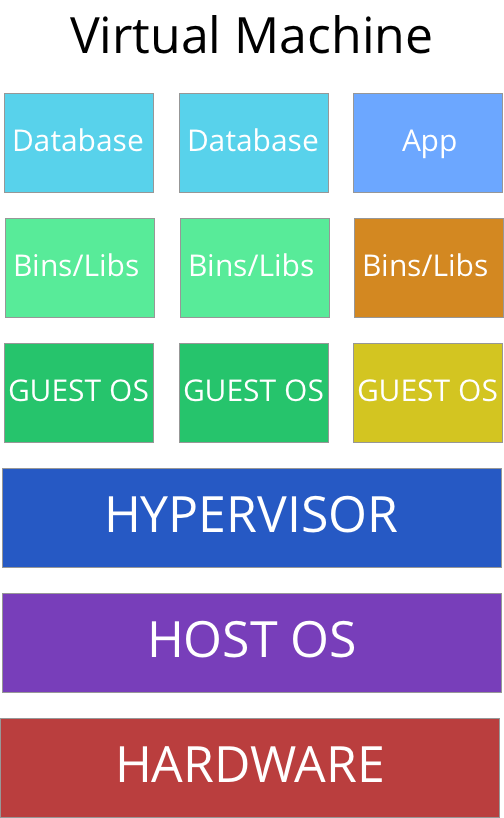
\includegraphics[width=3cm]{img/virtual-machine}
    \caption{structuur van een virtuele machine}
    \label{fig:virtualmachine}
\end{wrapfigure}

Het concept van virtualisatie deelt een aantal gelijkenissen met timesharing. De computer wordt opgedeeld in verschillende delen bij virtualisatie. Bij timesharing wordt de computer opgedeeld in afzonderlijke contexten.

Een aantal voordelen van virtualisatie zijn de volgende: financieel voordeel (men kan van één taak naar meerdere taken gaan op één computer), het besparen van energie (\cite{beloglazov_energy_2010}) en veiligheid(\cite{mortleman_security_2009}).

Een virtuele machine (\cite{smith_architecture_2005}) bootst een computer na. Een virtuele machine kan de middelen van de fysieke computer, waar het zich op bevindt, gebruiken. Dit zorgt ervoor dat de middelen van de fysieke computer kunnen gebruikt worden als virtuele middelen. Doorheen deze bachelorproef zal naar de fysieke computer verwezen worden als de host machine. Guest is de naam dat wordt gegeven aan virtuele machines die zich bevinden op de host. In het volgende deel zullen we de laag tussen de host machine en virtuele machine bekijken: de hypervisor. Figuur \ref{fig:virtualmachine} toont de structuur van een virtuele machine. 

\section{Hypervisor}

Een hypervisor (\cite{popek_formal_1974}) is een voorbeeld van hardware virtualisatie. Het is een stuk software, firmware of hardware, dat de laag vormt tussen de virtuele machine en de host machine. De host machine zorgt voor de middelen zoals CPU, RAM, enzoverder. Elke virtuele machine die zich bevindt op de host machine zal dan gebruik kunnen maken van een gedeelte van deze middelen. Doordat virtualisatie alomtegenwoordig geworden is in datacenters (\cite{soundararajan_impact_2010}) heeft het ervoor gezorgd dat er meer logica komt te liggen bij de hypervisor. De hypervisor neemt verder de rol op zich van het verdelen van de middelen en het beheren van de guests. Er zijn twee soorten hypervisors: type 1 en type 2. Type 1 is de bare-metal hypervisor en type 2 de hosted hypervisor.

\newpage

\subsection{Hosted Hypervisors}

\begin{wrapfigure}{r}{0.3\textwidth}
    \centering
    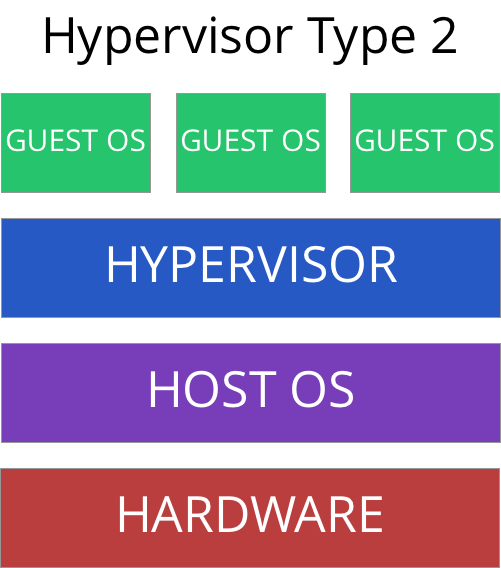
\includegraphics[width=3cm]{img/hypervisor-2}
    \caption{structuur van een hosted hypervisor}
    \label{fig:hypervisor-2}
\end{wrapfigure}

Als eerste zullen we de hosted hypervisor of type 2 hypervisor behandelen. Figuur \ref{fig:hypervisor-2} toont de structuur van een hosted hypervisor. De hosted hypervisor bevindt zich op het besturingssysteem van de host machine en heeft geen directe toegang tot de hardware. De type 2 hypervisor is dus compleet afhankelijk van het besturingssysteem van de host om zijn taken uit te voeren. Als er problemen optreden in het besturingssysteem van de host heeft dit gevolgen voor de hypervisor en guests.

Voorbeelden van hosted hypervisors zijn: Oracle Virtualbox (\cite{oracle_oracle_2016}) en VMware Workstation (\cite{vmware_vmware_2016}).

\subsection{Bare-metal Hypervisors}

\begin{wrapfigure}{l}{0.3\textwidth}
    \centering
    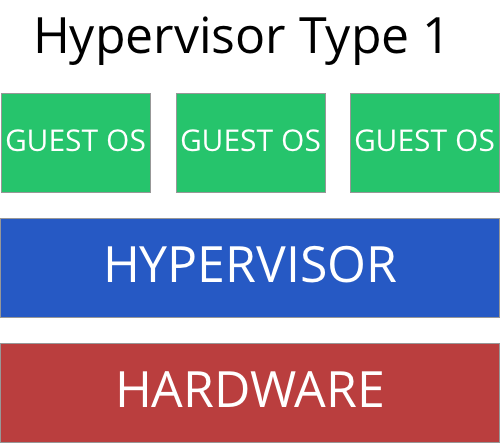
\includegraphics[width=3cm]{img/hypervisor-1}
    \caption{structuur van een bare-metal hypervisor}
    \label{fig:hypervisor-1}
\end{wrapfigure}

Type 1, bare-metal, embedded of native hypervisors bevinden zich rechtstreeks op de hardware. De voornaamste taak van de hypervisor is het beheren en verdelen van middelen. Dit maakt de hardware hypervisor kleiner in omvang dan de hosted hypervisor. De hosted hypervisor is niet afhankelijk van het besturingssysteem van de host machine want de hosted hypervisor bevindt zich rechtstreeks op de hardware. Figuur \ref{fig:hypervisor-1} toont de structuur van een bare-metal hypervisor.

Er is een laag minder in de structuur dus dit betekent dat er minder instructies moeten worden uitgevoerd bij een bepaalde handeling. Dit heeft een betere prestatie tot gevolg. Omdat er geen problemen kunnen zijn met het besturingssysteem van de host kan er aangenomen worden dat deze soort hypervisors stabieler zijn. Wanneer het besturingssysteem van de host faalt bij een hosted hypervisor dan zal dit gevolgen hebben voor de guests.

Een paar voorbeelden van bare-metal hypervisors zijn VMware ESXi en Xen.

\section{Operating System-level Virtualisation}

Naast hardware virtualisatie kan ook een besturingssysteem gevirtualiseerd worden. Bij deze toepassing van virtualisatie worden de mogelijkheden van de kernel gebruikt. De kernel van bepaalde besturingssystemen laat toe om meerdere geïsoleerde namespaces tegelijkertijd te laten werken. Dit zorgt ervoor dat er maar één besturingssysteem moet zijn om verschillende programma's naast elkaar en geïsoleerd te laten werken.

Elke namespace heeft zijn eigen configuratie en zijn geïsoleerd van elkaar. Dit geeft eveneens de beperking dat de guests over een besturingssysteem of kernel moeten beschikken, die overeenkomt met de host.

Tegenover hardware virtualisatie zal besturingssysteem virtualisatie minder gebruik maken van middelen omdat er maar één besturingssysteem is. Dit is omdat het besturingssysteem wordt gedeeld. Dit geeft voordelen bij de prestatie.

Voorbeelden van besturingssysteem virtualisatie zijn: chroot (\cite{linux_chroot2_????}), Solaris Containers (\cite{oracle_solaris_2016}) en Docker (\cite{docker_docker_2016}).

Besturingssysteem virtualisatie is vooral bekend geworden door Docker vanaf 2013 (\cite{hykes_future_2013}). In het volgende hoofdstuk wordt verder ingegaan op besturingssysteem virtualisatie onder de vorm van software containers.

\chapter{Software Containers}
\label{ch:Containers}

\section{Software Containers}

\begin{wrapfigure}{l}{0.3\textwidth}
    \centering
    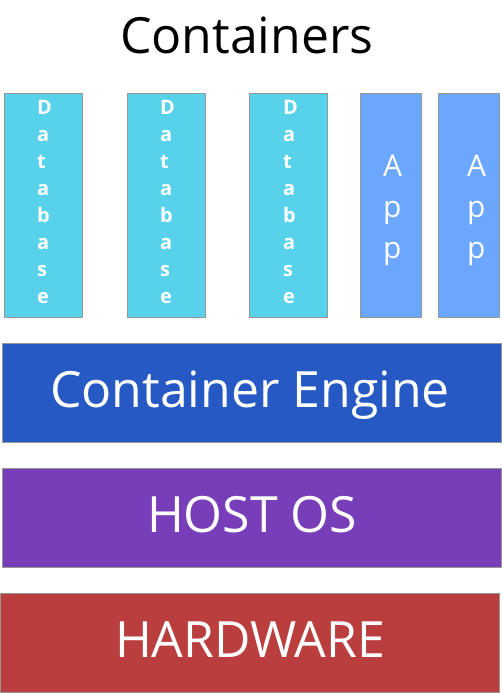
\includegraphics[width=3cm]{img/container}
    \caption{structuur van containers}
    \label{fig:containers}
\end{wrapfigure}

Software containers bestaan al een ruime tijd. In \cite{soltesz_container-based_2007} werd al gekeken naar de voordelen van software containers ten opzichte van hypervisors. Chroot (\cite{_linux_????}) is een concept dat veel deelt met sofware containers. Chroot zal de root directory van het huidige proces en zijn children veranderen. Er wordt een virtuele kopie gemaakt van het systeem waarin het proces kan werken. Het proces is dus afgesloten van het systeem en dit zorgt voor meer veiligheid bij het uitvoeren van processen.

Linux Containers of LXC (\cite{containers_linux_????}) is een implementatie van besturingssysteem virtualisatie. LXC kan meerdere geïsoleerde Linux systemen laten werken op één host. Deze geïsoleerde Linux systemen worden sofware containers genoemd. Deze containers worden ook getoond in figuur \ref{fig:containers} waarbij de apps en databases containers zijn.

Zoals al gezien is, is de rol van de hypervisor het delen en beheren van de middelen. Om containers te gebruiken, moet een ander deel de rol van de hypervisor overnemen. Cgroups is een Linux kernel extension die deze rol overneemt. Door middel van cgroups kunnen middelen worden beheerd voor processen. Het toont ook de mogelijkheden om backups te creëren van processen.

Eerder werd ook al aangehaald dat de processen van elkaar gescheiden moeten worden. Dit wordt bereikt door namespaces. De functies die name spaces voorzien zijn uitgebreid. Elke namespace heeft zijn eigen bestandssysteem structuur, netwerk interfaces en proces ID space. De containers delen de kernel met alle andere processen die op de kernel aan het werken zijn.

De containers zijn van elkaar afgesloten. Wanneer één container aangetast wordt, dan heeft dit geen rechtstreeks gevolg op de andere containers.

Toch zijn er een paar andere problemen zoals aangehaald in \cite{madhavapeddy_jitsu:_2015}. Processen die als root werken kunnen niet geïsoleerd worden van elkaar. Verder wordt er ook aangehaald dat strengere isolatie nodig is. (tabel 2, \cite{madhavapeddy_jitsu:_2015})

\section{Docker}

Docker (\cite{docker_docker_2016}) is een open source project om software containers te gebruiken voor programma's gemakkelijk te ontwikkelen en te laten werken op verschillende besturingssystemen.

Er zijn andere formaten zoals rkt \cite{_rkt_????} die het ook mogelijk maken om gemakkelijk software containers te gebruiken.

In 2015 werd het Open Container Initiative opgericht. Veel grote spelers op vlak van software containers zoals Docker, CoreOS, Microsoft en Google maken hier deel van uit. Samen willen ze een standaard voor software containers vastleggen. \cite{}.

De problemen die we bij software containers tegenkomen hebben voornamelijk betrekking tot beveiliging. Unikernels kunnen een veiliger alternatief zijn. In het volgende hoofdstuk worden de werking en mogelijkheden met unikernels bekeken.

\chapter{Unikernels}
\label{ch:unikernels}

\section{Inleiding}

Dit hoofdstuk zal uitleggen uit welke delen een unikernel bestaat. Tevens wordt er ook beeld gegeven over de voordelen en eigenschappen van unikernels. In het volgende hoofdstuk wordt bekeken welke implementaties van unikernels er al bestaan en wat de verschillen tussen deze implementaties zijn.

Virtuele machines (hoofdstuk \ref{ch:virtualisatie}) zijn er gekomen wanneer men de middelen van computers beter wou gebruiken. Toch werden de middelen niet optimaal benut door de besturingssystemen die werden gebruikt. Bij containers (hoofdstuk \ref{ch:Containers}) wordt het besturingssysteeem van de host machine gedeeld tussen de verschillende software containers. De middelen worden efficiënter gebruikt, doordat er maar één besturingssysteem is.

Unikernels (\cite{madhavapeddy_unikernels_2013}) gaat een andere weg op. Bij unikernels wordt er gekeken naar het besturingssysteem. Traditionele besturingssystemen zoals Ubuntu worden onder de loep genomen. De meeste besturingssystemen die worden gebruikt binnen een productieomgeving, kunnen ook gebruikt worden voor algemene doeleinden.

De eerste implementaties van unikernels worden tegengekomen op het einde van de jaren 90. Exokernel (\cite{mit_mit_1998}) werd ontwikkeld door MIT. De software ontwikkelaars kunnen zelf dus keuzes maken op vlak van abstractie. Nemesis (\cite{university_of_cambridge_nemesis_2000}) werd vanuit de universiteit van Cambridge ontwikkeld. Deze onderzoekers wilden unikernels gebruiken voor doeleinden binnen de multimedia.

Unikernels vragen inzicht in een aantal verschillende technologiëen. De kernel ligt aan de basis van een besturingssysteem en zal in de volgende sectie worden uitgelegd.

\section{Kernel}

De kernel is het programma dat zich centraal bevindt in het besturingssysteem. Het werkt rechtstreeks met de hardware van de computer. De kernel kan gezien worden als het fundament waar het hele besturingssysteem op steunt. Omdat het een belangrijke rol vervult, in het besturingssysteem, is veel van het geheugen van de kernel beveiligd. Dit is bedoeld zodat bepaalde applicaties geen veranderingen kunnen aanbrengen in de kernel. Als er iets fout zou gaan met de kernel, dan heeft dit rechtstreekse gevolgen op het besturingssysteem. Al de handelingen die de kernel uitvoert bevinden zich in de kernel space. Daartegenover gebeurd allles wat de gebruiker uitvoert zich in de user space. Het is van uiterst belang dat de kernel space en user space strikt van elkaar gescheiden zijn. Als dit niet zo zou zijn, dan zou een besturingssysteem niet veilig zijn. De kernel voert nog andere taken uit zoals geheugenbeheer en system calls. Figuur \ref{fig:kernel} toont de positie van de kernel binnen het systeem.

\begin{wrapfigure}{r}{0.3\textwidth}
    \centering
    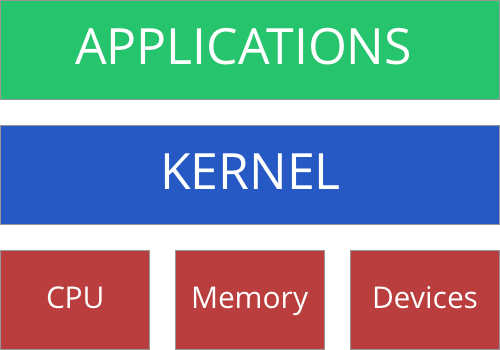
\includegraphics[width=3cm]{img/kernel}
    \caption{positie van kernel tussen de programma's en hardware}
    \label{fig:kernel}
\end{wrapfigure}

Als een programma wordt uitgevoerd, dan bevindt het programma zich binnen de user space. Om het programma in werkelijkheid te kunnen uitvoeren, moet er om toestemming gevraagd worden aan de kernel. Deze instructies moeten worden nagegaan voor de veiligheid. Soms wordt er ook gesproken van memory isolation, waarbij de user space en kernel space niet rechtstreeks met elkaar kunnen communiceren. Dit is een veiligheidsmaatregel.

Volgend boek heeft meer informatie over de werking van de kernel (\cite{bovet_understanding_2005}).

De twee volgende delen zullen de belangrijkste eigenschappen van unikernels uitleggen.

\section{Library besturingssysteem}

Elke virtuele machine binnen de architectuur van een productieomgeving heeft meestal één functie. Dit is al getoond in figuur \ref{fig:virtualmachine}. Elke guest heeft een gespecialiseerde rol om de middelen, dat het ter beschikking krijgt, optimaal te benutten.
Dezelfde architectuur en denkwijze kan teruggevonden worden bij containers. De besturingssystemen, die virtuele machines en containers gebruiken, kan traditioneel worden genoemd. Dit is aangehaald in \cite{madhavapeddy_unikernels_2013}.

Als er dieper wordt ingegaan op deze evolutie, dan kunnen we een patroon vaststellen: er worden steeds kleinere eenheden gebruikt. Eerst was de machine de eenheid en dan de virtuele machine. In het geval van software containers is de eenheid een container. Een unikernel kan ook bekeken worden als een eenheid binnen dit patroon.

Het meest gebruikte besturingssysteem voor servers is het Ubuntu besturingssysteem (\cite{matthias_gelbmann_ubuntu_2016}) met 32\%. Veel applicaties van databases tot en met web applicaties gebruiken het. Dit terwijl een database en een web applicatie andere middelen en functionaliteit nodig hebben.
Er zijn er ook gespecialiseerde besturingssystemen zoals Mini-OS (\cite{satya_popuri_tour_????}). Mini-OS gebruikt veel van de overbodige functies van een traditioneel besturingssysteem niet. Deze gespecialiseerde besturingssystemen zijn in de minderheid en ook niet zeer gekend.

Traditionele besturingssystemen zijn niet de basis die men nodig heeft in een architectuur waar elke eenheid één rol heeft. Alpine (\cite{alpine_linux_development_team_alpine_????}) is een Linux besturingssysteem dat een zeer minimale basis heeft. Tevens beschikt het over een uitgebreide package repository. Dit maakt het een ideaal besturingssysteem voor de basis van software containers. Er kan gestart worden met een kleine basis en alle onderdelen toevoegen die nodig zijn. Dit zorgt voor een container met een kleinere omvang. Hier wordt verder over uitgeweid in sectie \ref{sec:bene_unikernels}.

\begin{wrapfigure}{r}{0.4\textwidth}
    \centering
    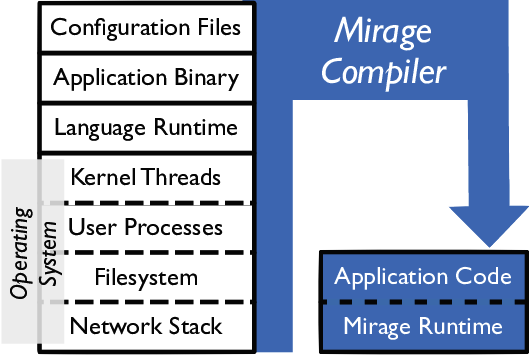
\includegraphics[width=6cm]{img/unikernel}
    \caption{algemeen besturingssysteem tegenover een unikernel implementatie \cite{madhavapeddy_unikernels_2013}}
    \label{fig:unikernel}
\end{wrapfigure}

Sommige onderdelen van het besturingssysteem hebben geen nut meer. Dit kan voor slechtere prestaties en lagere veiligheid zorgen.

Het concept van library besturingssystemen (\cite{madhavapeddy_unikernels_2013}) neemt dit nog een stap verder. Er wordt met een absoluut minimale basis gestart. Daarna worden alleen de componenten toegevoegd, die nodig zijn voor de functionaliteit die de eenheid uitvoert. Library duidt op de verschillende onderdelen of componenten die kunnen worden toegevoegd.

Web applicaties hebben verschillende functies nodig om te kunnen communiceren. Hiervoor bestaan netwerkprotocollen. TCP is een kritiek protocol om te communiceren met het internet en andere apparaten. Bij algemene besturingssystemen, zoals Ubuntu, is dit al aanwezig. Omdat er gestart wordt met een minimale basis, moeten deze protocollen geïmplementeerd worden. Gelukkig zijn er libraries die hiervoor kunnen gebruikt worden. De libraries, broncode en configuratie worden dan gecompileerd. Als resultaat heb je dan een image. Wanneer deze image wordt uitgevoerd dan hebben we een werkende unikernel. De unikernel wordt gecompileerd voor één omgeving en kan alleen gebruikt worden op deze omgeving. Dit is een verschil met software containers en virtuele machines die meer los staan van de omgeving waarin ze zich bevinden.

Unikernels kunnen enkel werken op de omgeving waarvoor ze gecompileerd zijn. Dit is omdat drivers voor de hardware componenten moeten worden geschreven. Kleine veranderingen in de specificatie of interface van een hardware component zorgt ervoor dat de driver niet meer werkt. Drivers zijn één van de grootste obstakels die worden vastgesteld bij library besturingssystemen. Hypervisors lossen dit probleem op door een standaard interface open te stellen. Zo moet er alleen maar één driver worden geschreven voor de hardware component. het werk wordt uitermate verminderd door dit. De protocollen, waar eerder over gesproken is, vormt dan nog een deel van het werk.

\section{Single Address Space}

In een unikernel bestaat er geen concept van user of kernel space. Alle processen bevinden zich binnen dezelfde space. Dit zou problemen geven bij traditionele besturingssystemen. Maar bij het compileren van de unikernel wordt de broncode, libraries en configuratie gecontroleerd. Dit is om te kijken of er zich geen problemen kunnen voordoen. De afwezigheid van de communicatie tussen de kernel en user spaces zorgt voor betere prestaties. Deze verbetering van de prestatie komt ook doordat de hardware kan worden aangesproken zonder dat er veranderd moet worden van context.

Eén globale address space zorgt voor problemen met de isolatie van processen. Meerdere programma's naast elkaar laten werken op een library besturingssysteem is complex. De hypervisor lost dit probleem gedeeltelijk op. Een mogelijke oplossing voor dit probleem wordt verder besproken in Hoofdstuk \ref{ch:microservices}.

\section{Veiligheid}

De hoge mate van veiligheid van unikernels is een gevolg van de specialisatie van de eenheid. Bij virtuele machines en software containers zijn traditionele besturingssystemen de basis. Deze besturingssystemen hebben zeer veel functionaliteit die niet nodig is voor de specifieke taak dat ze uitvoeren. De overbodige functionaliteit kan zorgen voor een lagere prestatie, maar ook voor meer veiligheidsrisico's. Het is dus gemakkelijker om de veiligheid te garanderen van een kleinere broncode tegenover een grote. Daar komt nog bij dat er unikernel implementaties worden gebruikt die specifiek zijn voor de omgeving. Het vraagt veel meer moeite om een gespecialiseerde implementatie te schrijven tegenover een algemene implementatie. Het marktaandeel van de algmene implementatie zal ook veel groter zijn tegenover de specifieke implementatie.

Verder heeft een unikernel geen shell of een andere mogelijkheid om een unikernel aan te passen terwijl deze aan het werken is. Eén unikernel overnemen heeft geen gevolg op de andere unikernels. Daarbij komt nog dat de hypervisors zelf meer veiligheid garanderen (\cite{colp_breaking_2011}).

\section{Andere voordelen}
\label{sec:bene_unikernels}

De omvang van een unikernel is kleiner dan een virtuele machine of een container. Zoals er al eerder werd aangehaald kunnen containers ook een kleine omvang hebben wanneer ze een miniem besturingssysteem gebruiken. Een voorbeeld daarvan is Alpine dat start vanaf 5 MB (\cite{_gliderlabs/docker-alpine_????}).
Een voorbeeld van de omvang van een unikernel kan gevonden worden in \cite[hoofdstuk 4, p.~10]{madhavapeddy_jitsu:_2015} met 1 MB.

Het systeem optimaliseren kan ook in veel grotere mate gebeuren (\cite{madhavapeddy_turning_2010}) dan bij traditionele besturingssystemen.

\section{Productie}

Veel van de commentaar die gegeven wordt op unikernels komt van de moeilijkheden om te kijken wat er fout gaat in productie (\cite{bryan_cantrill_unikernels_2016}). Aanpassingen doen in productie om problemen te verhelpen is niet de beste manier om iets op te lossen. Het programma moet uitgebreid getest worden vooraleer het in de productieomgeving wordt opgesteld. Wanneer er dan toch iets fout gaat in productie, dan zal men de situatie proberen na te bootsen in een soortgelijke omgeving. Het terugzetten van een oudere versie van het programma kan helpen om de gebruikers geen ongemak te laten ondervinden.

\section{Hedendaags gebruik}

Unikernels kunnen momenteel gebruikt worden in beperkte situaties. Er was hetzelfde fenomeen te vinden bij software containers een paar jaar geleden, vooraleer Docker op de voorgrond trad. Elke technologie moet een bepaalde tijd ondergaan om matuur te worden.

In het volgende deel zullen we implementaties van verschillende unikernels vergelijken om een beter beeld te krijgen van de huidige mogelijkheden en het huidige landschap.

\chapter{Vergelijking implementaties unikernels}
\label{ch:vergelijking-unikernels}

\section{Inleiding}

In het hoofdstuk over unikernels zijn er een aantal voorbeelden van moderne implementaties van unikernels aangehaald. In dit hoofdstuk zullen er een aantal implementaties van unikernels worden vergeleken met elkaar. Het volgende deel zal aanhalen welke criteria, er zullen gebruikt worden om deze vergelijking te realiseren.

\section{Criteria}

\begin{description}
\item [Implementatie programmeertaal]
Op het eerste zicht lijkt de programmeertaal waarin de implementatie geschreven niet belangrijk. Dit is wel belangrijk om te weten of het een programmeertaal is waar gemakkelijk kan mee gewerkt worden.
Een meer voor de hand liggende programmeertaal, zoals C++, zal gemakkelijker open source ontwikkelaars aantrekken. En dat is ook een belangrijk gegeven.
De meeste implementaties zijn in C/C++ geschreven. Dit komt vooral door het feit dat veel software ontwikkelaars die zich bezig houden met unikernels vanuit een achtergrond met besturingssystemen komen.
De meest gebruikte programmeertaal binnen besturingssystemen is C/C++.

\item [Hypervisors] 
Hypervisors zijn een groot deel van de keuze van een implementatie. De meest gebruikte unikernels zijn beschikbaar op een aantal hypervisors. Als er veel omgevingen zijn, waarop de unikernels kunnen werken, dan is het gemakkelijk om van omgeving te veranderen als bedrijf. Wendbaarheid en inspelen op veranderingen zal gemakkelijker gebeuren, wanneer er een uitgebreid aantal mogelijkheden zijn.

\item [Ondersteunde programmeertalen]
Sommige unikernels ondersteunen een aantal programmeertalen. Programmeertalen hebben sterke en zwakke kanten en keuze hebben uit een aantal programmeertalen helpt voor een keuze te maken.

\item [GitHub stars] 
GitHub bepaalt de status van een open source project. Open source software wordt meer en meer gebruikt door bedrijven. De keuze is gemakkelijker te maken tussen een project met een hoge populariteit(sterren) en een project met lage populariteit. Hierbij wordt er wel gesproken over projecten met dezelfde functionaliteit. Door GitHub kan gekeken worden of er actief aan het project gewerkt wordt en/of het onderhouden wordt. De community achter een project is ook belangrijk voor de keuze te maken tussen verschillende projecten.

\end{description}

\begin{sidewaystable}[ht]
\caption{Implementaties unikernels}
\begin{center}
    \begin{tabular}{| l | l | l | l | l |}
    \hline
    Naam & Taal implementatie & Hypervisor & Ondersteunde talen & GitHub sterren \\ \hline
    ClickOS & C/C++ & Xen & bindings & 243 \\ \hline
    HaLVM & Haskell & Xen & Haskell & 665 \\ \hline
    LING & C/Erlang & Xen & Erlang & 523 \\ \hline
    Rumprun & C & hw, Xen, POSIX & C, C++, Erlang, Go, ... & 469 \\ \hline
    MirageOS & OCaml & Xen & OCaml & 657 \\ \hline
    IncludeOS & C++ & KVM, VirtualBox & C++ & 1341 \\ \hline
    OSv & C/C++ & KVM, Xen, ... & JVM & 2121 \\ \hline
    \end{tabular}
\end{center}
\label{tab:impl_unikernels}
\end{sidewaystable}

De inhoud van de bovenstaande tabel wordt per implementatie uitgelegd en is te vinden op het einde van dit hoofdstuk.

\newpage

\section{Implementaties van moderne unikernels}

\subsection{ClickOS}
\begin{description}
  \item [Implementatie programmeertaal]: C/C++
  \item [Hypervisors]: Xen
  \item [Ondersteunde programmeertaal]: ondersteund door bindings
  \item [GitHub stars]: 243
\end{description}

ClickOS  (\cite{martins_clickos_2014}) wordt ontwikkeld door Cloud Networking Performance Lab.

De toepassingen, waarvoor ClickOS voornamelijk wordt gebruikt, zijn middlebox applicaties. Een middlebox is een netwerk applicatie dat netwerktrafiek kan omzetten, filteren, inspecteren of manipuleren. Voorbeelden hiervan zijn firewalls en load balanceres.
Een modulaire router vormt de basis van ClickOS. Op deze router kunnen onderdelen worden toegevoegd. Deze unikernel werkt alleen op MiniOS. MiniOS is beschikbaar bij de broncode van de Xen hypervisor.

Door een evolutie binnen de netwerk laag (\cite{garcia_villalba_trends_2015}) wordt veel van de functionaliteit, die vroeger bij de hardware zat, nu in software geïmplementeerd. Dit laat toe om een eigen implementatie te schrijven en zo veel functionaliteit van de hardware over te nemen.

De use cases waarbinnen ClickOS kan gebruikt worden zijn beperkt. Als je geen gebruik wilt maken van ingebouwde netwerk functionaliteit van de hardware, dan is ClickOS de uitgesproken keuze.

Er wordt Swig gebruikt om ondersteuning te bieden voor hogere programmeertalen. Swig maakt een bindings die C/C++ verbindt met een hogere programmeertaal.

ClickOS verwijst naar zijn packages als elements. Die elements voeren een bepaalde actie uit. Dit zijn hele kleine stukken functionaliteit. Er zijn om en bij de 300 elementen beschikbaar. Het is eenvoudig om zelf een eigen element te maken en te distribueren.

Meer informatie kan gevonden worden volgende website: \cite{cloud_networking_performance_lab_cloud_????}.

\subsection{HaLVM}

\begin{description}
  \item [Implementatie programmeertaal]: Haskell
  \item [Hypervisors]: Xen
  \item [Ondersteunde programmeertaal]: Haskell
  \item [GitHub stars]: 665
\end{description}

HaLVM (\cite{galois_inc._haskell_????}) wordt ontwikkeld door Galios. Galios is een software ontwikkelingsagentschap dat unikernels al een tijd in productie gebruikt.
Er zijn niet al te veel bedrijven die unikernels gebruiken in productie.

De programmeertaal waarin de unikernel van HaLVM wordt geschreven is Haskell. Haskell is een functionele programmeertaal met een uitgebreid type system. HaLVM is een implementatie die één supervisor en één programmeertaal ondersteunt.

Het werd ontwikkeld met als doel om componenten voor besturingssystemen snel te maken en te testen. Het is verder geëvolueerd naar andere use cases.

Bij HalVM wordt de Xen hypervisor als omgeving gebruikt. Er is een integratie met de Xen hypervisor waarvan de core library van HaLVM gebruikmaakt. Er bestaat ook een communicatie library, die bestaat uit het Haskell File System en de Haskell Network Stack. Deze library kan gebruikt worden in de meeste gevallen, als er netwerkfunctionaliteit nodig is. Als we meer mogelijkheden nodig hebben voor een programma dan kunnen er modules worden toegevoegd. Er is een ecosysteem uitgebouwd om het gemakkelijker te maken voor software ontwikkelaars om hun eigen modules te bouwen.

De werkwijze is de volgende: eerst wordt er zoveel mogelijk functionaliteit als een normaal Haskell programma geschreven. Daarna moet het programma aangepast worden om het te gebruiken op HaLVM.
Dit is niet gemakkelijk bij uitgebreide applicaties, want er zijn maar beperkte debug mogelijkheden op HalVM.

Zoals in de meeste gevallen moet de compiler van Haskell worden aangepast om de unikernel te maken. Het is ook geen probleem om standaard Haskell libraries in de code te gebruiken.

Het wordt gebruikt door Galios in productie en dit maakt het gemakkelijk om vragen te stellen. De GitHub repository, waar de applicatie zich op bevindt, is over het algemeen actief en is populair voor maar één programmeertaal te ondersteunen.

\subsection{Ling}

\begin{description}
  \item [Implementatie programmeertaal]: C/Erlang
  \item [Hypervisors]: Xen
  \item [Ondersteunde programmeertaal]: Erlang
  \item [GitHub stars]: 523
\end{description}

Ling (\cite{erlang_on_xen_cloudozer/ling_????}) is een Erlang virtuele machine die werkt op de Xen hypervisor. Het bedrijf achter Ling is Cloudozer. Ze hebben al meerdere language runtimes gemaakt die rechtstreeks op Xen werken.
Ling is open source maar de andere tools, onder meer het beheren van unikernels, zijn niet open source. Wanneer er problemen met het ecosysteem zijn, moet de ondersteuning van Cloudozer gecontacteerd worden.

Zoals bij HaLVM, moet de applicatie eerst worden geschreven in Erlang. De package manager die gebruikt word met Erlang is Rebar, dit is de standaard Erlang package manager. Na het omzetten van de applicatie naar een Xen afbeelding zou de unikernel moeten werken.

Railing is een tool die meegeleverd is met Ling die je toelaat om, erlang on Xen, afbeeldingen te maken. We gebruiken ook xl utility van Xen om domeinen te beheren.
De focus van Erlang on Xen is de Xen hypervisor. 

Bij het uitbrengen van een nieuwe versie van LING is het mogelijk geworden om andere omgevingen te ondersteunen. Dit heeft veel nieuwe omgevingen, zoals internet of things en mobiele omgevingen, mogelijk gemaakt.
Unikernels kunnen handig zijn op deze omgevingen omwille van de kleine omvang. 

Verder opent dit ook de mogelijkheid voor de unikernels van LING op bare-metal te laten werken.

\subsection{Rumprun}

\begin{description}
  \item [Implementatie programmeertaal]: C
  \item [Hypervisors]: hardware, Xen, KVM
  \item [Ondersteunde programmeertaal]: onder meer C, C++, Erlang, Go, Javascipt, Python, Ruby
  \item [GitHub stars]: 469
\end{description}

Rumprun  (\cite{_rumpkernel/rumprun_????}) gebruikt rump kernels voor hun implementatie. Deze rump kernels worden samengesteld uit componenten afkomstig van NetBSD. NetBSD is een traditioneel besturingssysteem maar is modulair geschreven. Men kan het dus gebruiken om een rump kernel samen te stellen.

Er is een uitgebreide keuze aan hypervisors waaruit kan gekozen worden. De term hw duidt op hardware. Dit betekent dat rumprun één van de enige implementaties is die rechtstreeks kan werken op hardware. De unikernel kan ook werken op besturingssystemen die een POSIX-interface hebben. De POSIX-interface duidt op de meeste Unix systemen.

Er zijn verschillende soorten implementaties van unikernels. Sommige unikernels specialiseren op basis van programmeertaal en andere op basis van omgeving. Sommige doen zelf beide. Rumprun behoort tot de laatste groep. Dit is wel niet zonder gevolg. De prestatie zal niet die van een gespecialiseerde unikernel kunnen evenaren.

De rump-run packages zijn implementaties van drivers, protocollen en libraries die kunnen toegevoegd worden aan de rumprun kernels. Er zijn een groot aantal packages die kunnen gebruikt wordenen de meest bekende zijn aanwezig.
Het spijtige is wel dat er nog geen packaging systeem aanwezig is. Dit zou er wel voor zorgen dat er gewerkt kan worden met verschillende dependencies en versies van packages.

Rumprun verziet zelf geen compiler. Er wordt gebruik gemaakt van een compiler die aanwezig is op het systeem. In het geval van Mac OS X moet er een aparte compiler geïnstalleerd worden.

De programmeertalen die ondersteund zijn, zijn de volgende: C, C++, Erlang, Go, Javascript(node.js), Python, Ruby en Rust.

Meer informatie is te vinden in volgende thesis: \cite{kantee_flexible_2012}.

\subsection{MirageOS}

\begin{description}
  \item [Implementatie programmeertaal]: OCaml
  \item [Hypervisors]: Xen, Unix
  \item [Ondersteunde programmeertaal]: OCaml
  \item [GitHub stars]: 657
\end{description}

Er kan gezegd worden dat het voor een deel allemaal begon bij MirageOS (\cite{mirage/mirage_0000}). Hun paper (\cite{madhavapeddy_unikernels_2013}) over unikernels en MirageOS wakkerde veel interesse aan. Ervoor was er wel al sprake van unikernels, maar MirageOS zorgde voor veel nieuwe initiatieven.

MirageOS is een cloud besturingssysteem gemaakt om veilige netwerk toepassingen, met een hoge prestatie, te maken op verschillende omgevingen.

De programmeertaal dat gebruikt word om een MirageOS applicatie te maken is OCaml.
OCaml is de algemene implementatie van de Caml programmeertaal en voegt object georiënteerd programmeren toe. Het wordt extensief gebruikt door Facebook. Deze taal is niet bekend en dit kan ervoor zorgen dat het niet veel tractie krijgt.

De voornaamste redenen om OCaml te gebruiken zijn static type checking en automatic memory management. De eerste reden is om tegen te gaan, dat er iets fout gaat wanneer een programma aan het werken is. De compiler gaat kijken of het geen onveilige code kan vinden. Als dit het geval is, wordt het programma niet gecompileerd.
Memory management is belangrijk voor resource leaks tegen te gaan. Resource leaks kunnen ervoor zorgen dat het programma meer middelen gebruikt dan het nodig heeft. In het extreme geval kan het systeem waarop het programma werkt ook hinder ondervinden van dit probleem.

De applicatie kan geschreven worden op een Linux of Mac OSX besturingssysteem. Deze applicatie kan dan werken op een Xen of Unix omgeving. Dit geeft veel mogelijkheden op het vlak van omgevingen. Er zijn plannen om mobiele omgevingen te ondersteunen.

MirageOS bestaat al een tijd en heeft een groot aantal libraries ter beschikking. Het heeft een uitstekende toolchain voor het compileren van programma's en het debuggen van de resulterende unikernel. Debuggen kan soms tot problemen leiden bij unikernels, want er kan niet in de unikernel gekeken worden welke problemen zich voordoen. Dit komt omdat de unikernel geen shell heeft. De debug optie kan hierbij helpen.

\subsection{IncludeOS}
\begin{description}
  \item [Implementatie programmeertaal]: C/C++
  \item [Hypervisors]: KVM, VirtualBox
  \item [Ondersteunde programmeertaal]: C++
  \item [GitHub stars]: 1341
\end{description}

IncludeOS (\cite{oslo_and_akershus_university_college_hioa-cs/includeos_????}) is gemotiveerd door het paper van \cite{bratterud_maximizing_2013}. Het onderscheid tussen een minimale virtuele machine tegenover een unikernel is zeer klein. Daarom worden beide termen afwisselend gebruikt. Net zoals ClickOS moeten de applicaties geschreven worden in C++.

IncludeOS zorgt voor een bootloader, standaard libraries, modules voor de drivers te implementeren en een build- en uitrolsysteem. Het is simpel om applicaties te maken voor deze unikernel. Je moet alleen één dependency toevoegen aan het programma. Dan kan het worden omgezet naar een unikernel. Er veranderd dus niet veel voor de software ontwikkelaars. Dit zorgt voor een vlotte overgang en dit is zeker belangrijk wanneer er gekozen wordt om applicaties te bouwen voor unikernels.

Meerdere processen tegelijk laten werken op een unikernel van includeOS is niet mogelijk. Dit kan sommige software ontwikkelaars afschrikken. Het gebruik van microservices (hoofdstuk \ref{ch:microservices}) is nog niet wijdverspreid en kan een factor zijn bij het selecteren van een unikernel implementatie. Enerzijds gaan bedrijven nooit bij unikernels uitkomen, wanneer hun architectuur niet gebaseerd op microservices. Er zijn ook geen race conditions mogelijk, omdat er maar één proces mogelijk is.

Momenteel ligt de focus van IncludeOS voornamelijk op C++. Dit is een strategie dat kan helpen wanneer software ontwikkelaars zoeken naar een implementatie die een gemeenschap heeft. IncludeOS heeft een grote gemeenschap van C++ software ontwikkelaars. Hun doel is vooral om een soortgelijk Node.js te maken maar dan in efficiënt C++.

Er zijn geen plannen om hogere programmeertalen zoals Javascript te ondersteunen. Ook is IncludeOS niet POSIX compliant en dit kan voor problemen zorgen wanneer er extra functionaliteit moet worden toegevoegd.

Als omgeving focussen ze KVM en Virtualbox. Het is het dus gemakkelijk om een unikernel te testen op de ontwikkelomgeving. Als je services schrijft in C++ dan is IncludeOS een zeer goede keuze. Er kan meer informatie gevonden worden op de GitHub repository: \cite{oslo_and_akershus_university_college_hioa-cs/includeos_????}.

\subsection{OSv}

\begin{description}
  \item [Implementatie programmeertaal]: C/C++
  \item [Hypervisors]: VMWare, VirtualBox, KVM, Xen
  \item [Ondersteunde programmeertaal]: Java
  \item [GitHub stars]: 2121
\end{description}

OSv (\cite{cloudius-systems/osv_0000}) is een implementatie die een grote naam heeft binnen de unikernel wereld. Er wordt een hoog aantal programmeertalen ondersteund. Waaronder Java, Ruby, Javascript, Scala en vele anderen. Hierbij moeten er wel vermeld worden dat de implementaties van Ruby en Javascript in Java zijn geschreven. Rhino en JRuby zijn de namen van deze implemenaties. Het is simpel om deze programmeertalen toe te voegen, wanneer Java als programmeertaal wordt ondersteund.

Verder kunnen de resulterende unikernels werken op veel omgevingen: VMware, VirtualBox, KVM en Xen.

Zoals IncludeOS voorheen is OSv geschreven in C++.

Voor het beheren van een OSv instance kan gebruik worden gemaakt van de GUI. Bij de meerderheid van unikernels is informatie te vinden door middel van een GUI onmogelijk. Extensies voor de hypervisor kunnen hierbij helpen, maar dan nog komt de user experience tekort. De GUI is gebouwd op een REST API die de componenten van OSv openstellen. Dit heeft overstemming met de manier, hoe de architectuur van het Docker ecosysteem in elkaar zit. Deze componenten stellen een API open waar de tools verder op gebouwd kunnen worden. Er is een API-specificatie die kan bekeken worden om te zien hoe deze componenten met elkaar werken.

OSv ondersteund Amazon Web Services en Google Container Engine als cloud providers. Het is uitzonderlijk dat een unikernel zoveel informatie heeft over hoe het moet gebruikt worden. Er is documentatie over cloud providers, hypervisors, hoe het gebruikt moet worden en hoe programma's moeten omgezet worden naar de implementatie.

Het is de meest populaire implemenatie van unikernels van alle implementaties die we hebben overlopen tijdens deze vergelijking. Ook de activiteit op de Github repository is het hoogste van alle bekeken unikernels.

Meer informatie is te vinden in volgende paper: \cite{kivity_osvoptimizing_2014}.

\section{Conclusie}

Er zijn veel verschillende soorten implementaties van unikernels op dit moment. Er is MirageOS die als één van de eerste opkwam en ook de meest extreme weg opgaat met het starten van een minieme basis. HalVM bevindt zich in aan de dezelfde kant als MirageOS. Terwijl OSv en Rumprun zich bevinden aan de overkant. Ze ondersteunen een groot aantal programmeertalen en omgevingen. Dit wordt mogelijk gemaakt door een tussenlaag te gebruiken die zorgt voor compatibiliteit. 

Hetzelfde fenomeen kunnen we vinden met de toepassingen waar de unikernels kunnen voor gebruikt worden. ClickOS heeft vooral middlebox applicaties als doel en andere unikernels kunnen voor uiteenlopende situaties kunnen gebruikt worden.
\chapter{Microservices en monolieten}
\label{ch:microservices}

De meeste programma's worden gemaakt door een monolothische architectuur te hanteren (\cite{villamizar_evaluating_2015}). Alle functionaliteit en verantwoordelijkheden worden gestopt in één programma. Dit soort van programma wordt een monoliet of monolith in het Engels genoemd. De architectuur waarin deze soort programma's voorkomen noemen we een monolithische architectuur. Software ontwikkelaars structureren door middel van patronen (\cite{tichy_catalogue_1997}) om functionaliteit en verantwoordelijkheid van elkaar te scheiden. Modulariteit is hierbij een belangrijk gegeven.

\begin{wrapfigure}{r}{0.4\textwidth}
    \centering
    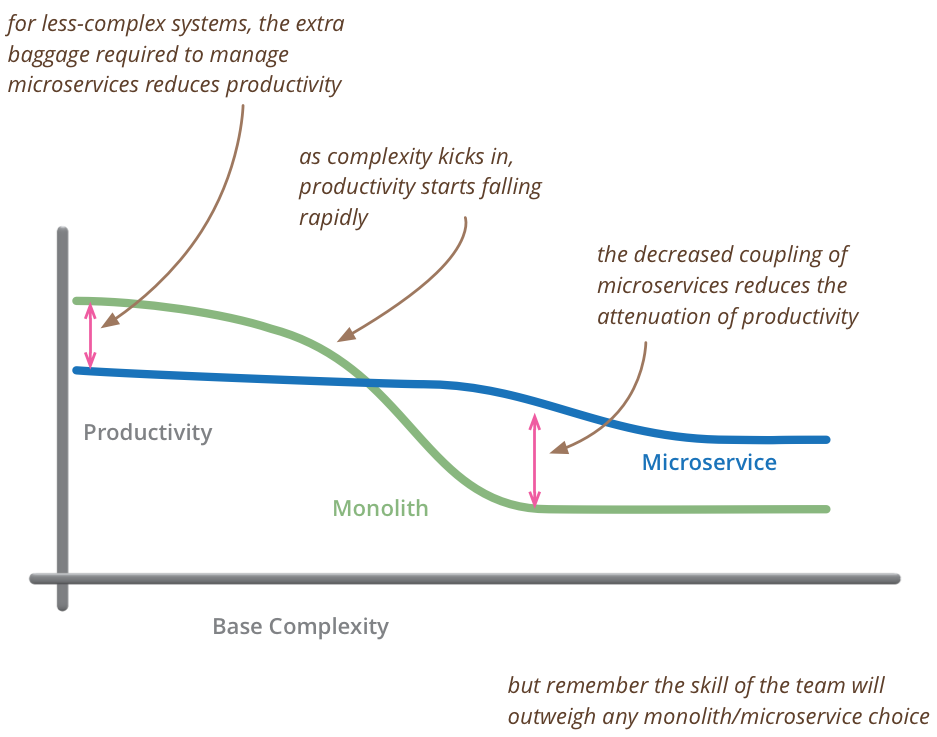
\includegraphics[width=6cm]{img/microservices_monolith}
    \caption{Productiviteit en complexiteit van microservices architectuur tegenover een monolithische architectuur (\cite{martin_fowler_microservicepremium_2015})}
    \label{fig:pr}
\end{wrapfigure}

Een probleem dat veel voorkomt bij een monolithische architectuur is dat het programma zeer complex wordt na verloop van tijd (\cite{villamizar_evaluating_2015}). Functionaliteit toevoegen is niet vanzelfsprekend bij een complex programma, want er moet rekening worden gehouden met de andere delen van het programma. Nieuwe software ontwikkelaars die het programma niet kennen moeten eerst een paar weken het programma verkennen. Dan pas kan er begonnen worden met nieuwe functionaliteit te schrijven.

Schaalbaarheid is een probleem waar ook tegen gelopen wordt na verloop van tijd (\cite{villamizar_evaluating_2015}). Sommige onderdelen van een programma moeten meer trafiek kunnen verwerken dan andere delen. Zoals al aangehaald werd in hoofdstuk \ref{ch:virtualisatie}, hebben verschillende soorten programma's andere middelen nodig. Dit is hetzelfde bij de interne delen van programma. Het schalen van deze componenten is alleen mogelijk door een nieuwe instantie toe te voegen van de hele applicatie of de implementatie te verbeteren. Eén groot programma is ook niet handig voor grote teams te laten samenwerken. Het uitbrengen van een versie moet dan nagegaan worden bij alle teams die aan dat programma werken.

Al langer bestaat het idee om een groot programma op te splitsen in kleinere programma's. Telecommunicatie is een industrie waarbinnen microservices al werden gebruikt \cite{griffin_survey_2007}. De opkomst van software containers heeft dit deze werkwijze meer verspreid. Dit komt omdat het gemakkelijker is geworden om kleinere programma's met elkaar te verbinden, zelf als ze zich niet op dezelfde omgeving bevinden. De architectuur waarbinnen dit idee wordt gebruikt, wordt microservices architectuur genoemd. De microservices kunnen we bekijken als deelapplicaties die één verantwoordelijkheid hebben.

\begin{wrapfigure}{r}{0.4\textwidth}
    \centering
    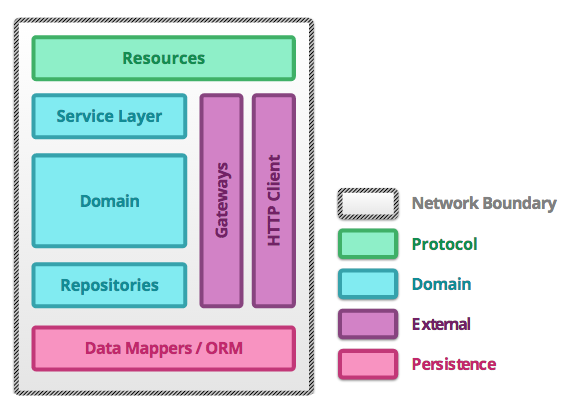
\includegraphics[width=6cm]{img/microservice_structure_example}
    \caption{Structuur van een architectuur met microservices (\cite{toby_clemson_testing_2014}) }
    \label{fig:microservice_structure_example}
\end{wrapfigure}


Een programma opsplitsen in componenten, met één verantwoordelijkheid, zorgt ervoor dat het meer schaalbaar is. Containers en unikernels helpen hierbij. Het opstarten van een nieuwe instantie van een microservice neemt minder tijd in beslag dan het opstarten van een nieuwe instantie van een monoliet.

Bij microservices zal de topologie van het probleemdomein goed gekend moeten zijn. Starten met het gebruiken van microservices architecture wanneer men het domein niet goed kent, vraagt om problemen. Het ontwerpen van een microservices architectuur moet goed gebeuren. Anders kunnen er problemen voorkomen met impact op de gehele architectuur, bijgevolg moeten er grote delen worden herschreven. Een monolietische architecture zal beter kunnen reageren op dit probleem. Als men later het domein kent kan een microservices architecture worden gebruikt. Hiervoor moet de monoliet modulair geschreven worden. Modulariteit is een vanzelfsprekende bouwsteen binnen programmeren.

De complexiteit van een monoliet wordt overgebracht naar het communiceren en het behouden van de consistentie tussen de microservices. Verder wordt ook het opstellen van de architectuur moeilijker.

Het voordeel van een microservices architecuur is dat de microservices van elkaar gescheiden zijn. Het gebruik van een nieuwe technologie of framework is niet langer een groot probleem. Dit komt omdat de microservices los van elkaar staan. Er kan dus een andere programmeertaal gebruikt worden zolang de communicatie tussen de microservices consistent blijft.

De communicatie van de microservices gebeurd via het netwerk. Dit maakt het mogelijk om microservices op verschillende virtuele machines of software containers te laten werken. Software defined network (\cite{garcia_villalba_trends_2015}) neemt veel complexiteit weg van de communicatie.

\begin{wrapfigure}{r}{0.4\textwidth}
    \centering
    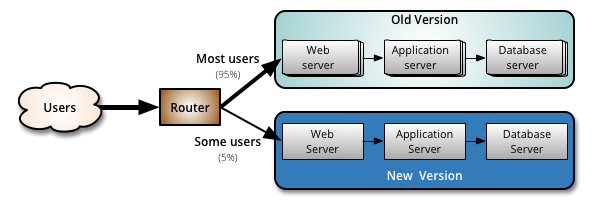
\includegraphics[width=6cm]{img/canary-release}
    \caption{Voorbeeld van een canary release (\cite{danilo_sato_canaryrelease_2014})}
    \label{fig:canary-release}
\end{wrapfigure}

Een monolietische architectuur opstellen in productie is relatief simpel tegenover een microservices architectuur. Wanneer er een nieuwe versie moet worden opgesteld in productie kan gebruik worden gemaakt van blue-green deployment (\cite{martin_fowler_bluegreendeployment_2016}). Waarbij we een oude en nieuwe versie hebben van de architectuur en de router het verkeer verlegt naar de nieuwe architectuur. Dit zorgt voor een gemakkelijke overgang.

Bij microservices kan gebruik gemaakt worden van een canary release strategie (\cite{danilo_sato_canaryrelease_2014}). Hier wordt weer een nieuwe versie opgesteld met de laatste veranderingen van de architectuur. De router gaat een deel van het verkeer naar de nieuwe architectuur versturen. Naarmate de tijd vordert, wordt het vertrouwen in de nieuwe versie nagegaan. Als het vertrouwen is toegenomen dan zal meer verkeer naar de nieuwe versie worden gestuurd. Zo kunnen er problemen worden nagegaan en er gepast op reageren. Uiteindelijk krijgt de oude versie geen verkeer meer en wordt alleen de nieuwe versie gebruikt.

De systeembeheerder krijgt meer werk omdat er nu tientallen microservices moeten beheerd worden in plaats van één grote applicatie. Het beheren van deze microservices en hun logs wordt een belangrijke bron van informatie binnnen de architectuur. Er kan gezegd worden dat deze microservices simpeler zijn om te verstaan, omdat de functionaliteit per microservices beperkt is. Sommige halen aan dat het de complexiteit die we niet meer tegenkomen in de applicatie nu terechtkomt bij het samen te laten werken van de verschillende onderdelen.

%%---------- Proof of concept -------------------------------------------------------------

\chapter{Proof of concept: unikernels in de praktijk}
\label{ch:proof-of-concept}
\section{Inleiding}

Dit hoofdstuk zal de toepassingen voor unikernels toelichten. De huidige implementaties van unikernels geven een zekere vrijheid wat voor soort applicaties er kunnen opgezet worden.  

Er kan gesproken worden over twee types van applicaties: dynamische en statische. Hiernaar wordt ook verwezen in het Engels als stateless en stateful. Blogs en websites zonder al te veel functionaliteit zijn stateless. Het resultaat van de applicatie qua functionaliteit zal hetzelfde zijn voor elke gebruiker. Stateful applicaties zijn web applicaties zoals Wordpress en de meeste applicaties waar er informatie wordt bijgehouden en kan worden aangepast. Het overgrote deel van de applicaties die werken met unikernels zijn stateless.

De verklaring hiervan is te vinden bij de eigenschappen van unikernels. Unikernels worden geoptimaliseerd voor de applicaties waarvoor ze gecompileerd worden. Het theoretische hoofdstuk over unikernels heeft hiervoor al de redenen gegeven. Wanneer de applicatie en een database zich op een unikernel bevinden dan zou de optimalisatie bijna geen voordelen geven. Daarbij komt er nog het extra gegeven van het opsplitsen van de verantwoordelijkheden van de componenten van een omgeving. Databanken vragen om een ander soort machine en/of besturingssysteem dan een webapplicatie. Hierbij is er nog het gegeven dat het bestaan van een relationele database nog niet bestaat voor unikernels onder een stabiele vorm. Irmin (verwijzing) kan wel een oplossing zijn, maar dit is moeilijk een relationele database te noemen. Ook kan Xenstore van de Xen hypervisor worden aangehaald. Dit levert dan weer het probleem op dat het niet op de verschillende soorten hypervisors kan gebruikt worden. Daarom kunnen databases zich beter bevinden op een virtuele machine met een algemeen besturingssysteem. Het probleem van databases en de correcte omgeving van databases kan ook teruggevonden worden bij software containers. Tot op het moment wordt aangeraden om databases te laten werken op virtuele machines omwille van de problemen met de levenstijd van software containers.

Veel van toepassingen die werken met unikernels bevinden zich meestal in een bepaald segment. Dit is het geval met technologieën die nog moeten toegroeien naar algemene of meerdere use cases. Toepassingen die moeten gebruik maken van unikernels zullen zich grotendeels bevinden binnen de netwerklaag. Rumprun heeft al pogingen gedaan om een soort van RAMP (RumpRun, Apache, MySQL, PHP) opstellingen te maken, maar dit staat nog in vroeg stadium. De functionaliteit laat hierbij te wensen over. Het maken van unikernels voor statische applicaties is dus een betere keuze voor de verschillende soorten unikernels te vergelijken.

\subsection{Keuze Programmeertaal}

Er worden een aantal programmeertalen ondersteund door unikernels. PHP, java, Node.JS, python, C++ en Go. Deze programmeertalen kunnen worden opgesplitst in twee groepen. Enerzijds zijn er de gecompileerde programmeertalen, zoals Go en C++, waarbij de broncode wordt omgezet in een uitvoerbaar bestand. Anderzijds kan er gesproken worden over geïnterpreteerde programmeertalen zoals PHP, java, Node.JS en python. Hierbij wordt de broncode door een interpreter vertaalt naar instructies die de processor kan begrijpen en de interpreter voert de instructies meteen uit. Het verschil is dus dat de compiler de instructies opslaat tegenover de interpreter die deze onmiddellijk uitvoert. Dit heeft een gevolg op de omgeving waarin de opstelling zich bevindt. Omwille van de aard van unikernels (beperkte levenstijd) kan een interpreter extra tijd innemen om de unikernel te starten. Enerzijds zou er gedacht kunnen worden dat dit een voordeel geeft aan de unikernels tegenover de software containers en virtuele machines. Maar de use cases waarbinnen unikernels kunnen worden gebruikt bevinden zich eerder in andere situaties. Voorbeelden hiervan zijn wanneer er uitzonderlijk geschaald moet worden of wanneer de unikernel de rol van een load balancer moet vervullen. 

Go zal gebruikt worden als programmeertaal om de applicaties te realiseren. Hieronder vind je een link naar deze programmeertaal.

\begin{description}
\item [Go] - https://golang.org
\end{description}

\section{Opstelling Virtuele Machine}

Deze opstelling maakt gebruik van Virtualbox als hypervisor met Vagrant, als configuratie tool, om de ontwikkelomgeving gemakkelijk op te stellen. 
De vereisten voor deze opstelling zijn:
\begin{description}
\item [Virtualbox] - https://www.virtualbox.org/
\item [Vagrant] - https://www.vagrantup.com/
\item [Repository Go Virtuele machine omgeving] - https://github.com/michieldewilde/vagrant-golang-bp
\item [Git] - https://git-scm.com/
\end{description}

Het besturingssysteem dat wordt gebruikt is Debian. De opstelling is simpel te noemen, omdat er enkel wordt uitgegaan van een applicatie die zich bevindt op de virtuele machine zonder andere componenten. In een productie omgeving zullen deze twee componenten zich uiteraard niet op dezelfde virtuele machine bevinden. Go wordt gebruikt als programmeertaal om de applicatie op de virtuele machine te demonstreren.

Allereerst is git nodig om de repository lokaal te downloaden. Git is een versie controle systeem om gemakkelijk grote en kleine projecten te beheren en te ontwikkelen wanneer er in team gewerkt wordt.

\noindent Het volgende commando zal de repository met de configuratie van de virtuele machine ophalen:
\begin{lstlisting}[language=bash]
  $ git clone https://github.com/michieldewilde/vagrant-golang-bp
\end{lstlisting}

De Vagrantfile in deze directory bevat de configuratie voor deze machine en zal ook zorgen dat de huidige directory van de host synchroniseert met de toegewezen directory in de virtuele machine.

\noindent Het volgende commando stelt de virtuele machine op en configureert deze:
\begin{lstlisting}[language=bash]
  $ vagrant up
\end{lstlisting}

\noindent Om deze virtuele machine te betreden wordt het volgende commando uitgevoerd:
\begin{lstlisting}[language=bash]
  $ vagrant ssh
\end{lstlisting}

Alle inhoud van de directory die we binnen hebben gehaald, bevindt zich op het /vagrant path. De programmeertaal Go heeft een structuur voor de projecten waarmee er wordt gewerkt. Er kan worden vastgesteld dat er in de directory die binnen is gehaald dat er een src directory aanwezig is. Binnen de src directory bevindt zich een main.go bestand. 

\noindent Om dit bestand uit te voeren:
\begin{lstlisting}[language=bash]
  $ go run main.go
\end{lstlisting}

Nu staat er een web server op en deze kan bereikt worden door in uw browser het IP van de virtuele machine in te geven, 192.168.10.10, en de poort 8080 met als prefix : er aan toe te voegen.

Bij deze is er een ontwikkelomgeving voor de programmeertaal Go opgesteld, met daarbij een web server. Het opstellen van een hele virtuele machine voor één applicatie kan overdreven lijken, maar daarbij zijn de vereisten voor de Go ontwikkelomgeving gescheiden van de host machine. Het toevoegen van extra onderdelen kan met gemak gebeuren door andere pakketten te installeren en te configureren. De functie van de virtuele machine die momenteel is opgezet is algemeen en kan gemakkelijk veranderen door onderdelen toe te voegen. Daarbij kan de virtuele machine met een algemeen besturingssysteem, Debian, beschouwd worden als niet gespecialiseerd. Dit is een uiteindelijk doel van elke component in de ontwikkelomgeving. 

\section{Opstelling Software Containers}

Deze opstelling maakt gebruik van Virtualbox als hypervisor met daarop Docker om de software containers te beheren en configureren.
De vereisten voor deze opstelling zijn:
\begin{description}
\item [Docker Toolbox] - https://www.docker.com/products/docker-toolbox
\item [Repository Go Software Container Omgeving] - https://github.com/michieldewilde/docker-golang-bp
\item [Simpele web server] - https://github.com/michieldewilde/go-web-example
\item [Git] - https://git-scm.com/
\end{description}

Er zijn al nieuwere versies van Docker uitgebracht voor specifieke besturingssystemen zoals Docker for Mac and Windows. Deze vertonen echter problemen bij het opstellen van unikerneles in het volgende hoofdstuk. Docker Toolbox laat toe om beide omgevingen te ondersteunen. Docker maakt het gemakkelijk om applicaties op te zetten in software containers.

\noindent Het volgende commando zal de repository met de configuratie van de software containers ophalen:
\begin{lstlisting}[language=bash]
  $ git clone https://github.com/michieldewilde/docker-golang-bp
\end{lstlisting}

Ga naar de opgehaalde directory en daarbinnen vindt uw een bestand genaamd Dockerfile, met alle configuratie die nodig is om een web server op te stellen binnen een software container.

\begin{lstlisting}[language=docker,caption={Dockerfile},breaklines=true,label={code:docker}]
FROM golang:1.6

# Haal de repository met het voorbeeld op
RUN go get github.com/michieldewilde/go-web-example

# Compileer het project
RUN go install github.com/michieldewilde/go-web-example

# Wanneer de software container wordt gestart, voer het gecompileerde project uit
ENTRYPOINT /go/bin/go-web-example

# Open poort 8080 om de web server te kunnen bereiken van op de host
EXPOSE 8080
\end{lstlisting}

Als Docker geïnstalleerd wordt dan wordt nog een extra tool mee geïnstalleerd: docker-machine. Deze tool laat toe om Docker hosts te creëren. Deze laat dan toe om met de Docker client die zich bevindt op de host te communiceren. 

Er zijn nog manieren om een meer uitgebreide en/of geavanceerde opstelling te bereiken dit kan bereikt worden door gebruik te maken van het docker-compose commando.

\begin{lstlisting}[language=docker-compose,caption={docker-compose.yaml},breaklines=true,label={code:docker-compose}]
# gebruik versie twee van de docker-compose syntax
version: '2'
# de verschillende componenten die moeten nodig zijn voor de opstelling
services:
  # onze simpele web server van de vorige voorbeelden
  go-web-example:
    # wanneer de service gecompileerd moet worden, gebruik de Dockerfile in de huidige directory (Dockerfile van het vorige voorbeeld)
    build: .
    # stel de pport 8080 open
    ports:
     - "8080:8080"
  # extra component voor database functionaliteit
  redis:
    image: "redis:alpine"
\end{lstlisting}

Door gebruik te maken van een docker-compose bestand wordt de opstelling van de verschillende componenten simpeler gemaakt. Ook het schalen van de componenten, wanneer er extra last wordt ondervonden, is ook gemakkelijker. Dit komt omdat de componenten gescheiden zijn van elkaar. Het toevoegen van extra componenten aan een opstelling kan dus gebeuren door een service toe te voegen aan het docker-compose bestand. Op de virtuele machine zou deze helemaal moeten worden geïnstalleerd en geconfigureerd worden. 

\section{Opstelling Unikernel}

Deze opstelling wordt uitgevoerd op een virtuele machine omdat er extensieve veranderingen worden uitgevoerd. Om deze opstelling lokaal te gebruiken zijn er drie vereisten nodig. Ten eerste de Virtualbox hypervisor. Verder Vagrant om de ontwikkelingomgeving op te stellen. Vagrant en Virtualbox gaan hand in hand om een start te maken wanneer er een bepaalde ontwikkelingomgeving nodig is. Vagrant werkt door middel van een bestand (VagrantFile). In dit bestand is alle configuratie van opstelling beschreven. Het haalt eerst een afbeelding op waarop de configuratie wordt toegepast. Packer is de laatste vereiste. Het zal gebruikt worden om op de virtuele machine de configuratie toe te passen. Dit resultaat wordt dan opgeslagen als een afbeelding.

\begin{description}
\item [Virtualbox] - https://www.virtualbox.org/
\item [Vagrant] - https://www.vagrantup.com/
\item [Packer] - https://www.packer.io/ 
\end{description}

Allereest moeten alle voorgenoemde vereisten zijn geïnstalleerd op uw machine voor er verder kan worden gegaan. MirageOS heeft een repository met alle benodigdheden om deze virtuele machine op te stellen. Deze kan gevonden worden op de volgende link: https://github.com/michieldewilde/mirage-vagrant-vms. Haal deze repository lokaal op de machine en navigeer naar de locatie van deze opgehaalde folder. Er is keuze uit ubuntu 14.04, ubuntu 14.10, debian 7.8.0 en xenserver 6.5.0. Er is gekozen voor Ubuntu 14.04 omdat er het minste problemen bij dit besturingssysteem zijn vastgesteld voor deze opstelling. De Makefile bevat gemakkelijkheidshalve commando's om de virtuele machine op te stellen zonder een lijst van commando's in te geven.

\noindent Het volgende commando zal een nieuwe box aanmaken door het gebruik van Packer:
\begin{lstlisting}[language=bash]
  $ make ubuntu-14.04-box
\end{lstlisting}

\noindent Het volgende commando neemt de box, die is aangemaakt door het vorige commando, en past de configuratie erop toe:
\begin{lstlisting}[language=bash]
  $ make ubuntu-14.04-box
\end{lstlisting}

\noindent Navigeer naar de folder van het gekozen besturingssysteem en ssh in de virtuele machine: 
\begin{lstlisting}[language=bash]
  $ cd ubuntu-14.04 && vagrant ssh
\end{lstlisting}

\subsection{MirageOS}

MirageOS is gestart vanaf nul met een schone lei. Dit betekende dat veel van de bestaande tools die nu worden gebruikt worden, zoals webservers (Apache, Nginx) en Databases (MySQL), herschreven zouden moeten worden. Het duurt een tijd voordat deze tervoorschijn komen en dit is één van de grootste redenen dat er gekozen is voor een statische applicatie.

De opstelling die gemaakt is in de vorige sectie heeft de toolset van MirageOS ook geïnstalleerd. Verder moet er worden gekeken of de juiste versie van Ocaml en OPAM (package manager) is geïnstalleerd:

\noindent OPAM versie:
\begin{lstlisting}[language=bash]
  $ opam --version
  # De versie moet minstens 1.2.2 zijn.
  1.2.2
\end{lstlisting}

\noindent Ocaml versie:
\begin{lstlisting}[language=bash]
  $ ocaml -version
  # Deze moet 4.02.3 of hoger zijn.
  $ opam switch 4.02.3
\end{lstlisting}

In de login shell moet de omgeving van opam ingeladen wanneer er ingelogd wordt. Dit kan gedaan worden door de volgende lijn toe te voegen aan het ~/.bashrc bestand:

\begin{lstlisting}[language=bash]
  $ eval `opam config env`
\end{lstlisting}

\noindent Verder moeten er ook gekeken of de versie van mirage niet moet aangepast moet worden:
\begin{lstlisting}[language=bash]
  $ opam install mirage
  $ mirage --help
  # Versienummer moet hoger zijn 2.9.0
\end{lstlisting}

Het mirage commando kan gebruikt worden om applicaties te maken en uit te rollen.

Als statische website zullen we de website van MirageOS zelf gebruiken. De repository van de website bevindt zich op de volgende link: https://github.com/mirage/mirage-www/. Eerst moet de repository worden opgehaald. 

\noindent Dit doen we door het git commando te gebruiken:
\begin{lstlisting}[language=bash]
  $ git clone https://github.com/mirage/mirage-www/
\end{lstlisting}

Vooraleer we de omgeving van de applicatie gaan configureren moet het mogelijk worden gemaakt om de Xen hypervisor te laten communiceren met de virtuele machine. Deze twee zijn afgeschermd van elkaar en daarom moet er een TUN/TAP constructie worden gemaakt. 

sudo modprobe tun
\noindent Dit doen we als volgt:
\begin{lstlisting}[language=bash]
  $ sudo apt-get install tunctl
  # laden van de tuntap kernel module
  $ sudo modprobe tun 
  # maak een tap0 interface
  $ sudo tunctl 

  $ sudo ifconfig tap0 10.0.0.1 up 
\end{lstlisting}

Navigeer naar de opgehaalde folder van de MirageOS website. 
\noindent Daarna moet de omgeving voor de applicatie worden ingesteld:
\begin{lstlisting}[language=bash]
  $ cd mirage-www
  $ make prepare
  $ cd src
  # configureren voor de Xen hypervisor
  # direct MirageOS network stack
  # maak gebruik DHCP
  $ mirage configure --xen \
      -vv --net direct \ 
      --dhcp true  \
      --tls false --network=0
\end{lstlisting}

Hierdoor is de omgeving van de applicatie goed ingesteld.
\noindent Het compileren van de unikernel gebeurd door middel van het volgende commando:
\begin{lstlisting}[language=bash]
  $ make
\end{lstlisting}

Eerst dienen er nog file blocks aangemaakt te worden om de afbeeldingen en de stylesheets te kunnen gebruiken:
\noindent Aanmaken file blocks
\begin{lstlisting}[language=bash]
  $ ./make-fat_block1-image.sh
\end{lstlisting}

Verder moeten er nog een paar wijzigingen worden aangebracht in het www.xl bestand. Dit bestand wordt doorgegeven naar de Xen launcher om de unikernel te starten.
\noindent Het disk gedeelte moeten worden aangepast naar het volgende:
\begin{lstlisting}
disk = ['format=raw,
         vdev=xvde,
         access=rw,
         target=/home/vagrant/mirage-www/src/fat_block2.img',
        'format=raw,
         vdev=xvdc,
         access=rw,
         target=/home/vagrant/mirage-www/src/fat_block1.img
      ']
\end{lstlisting}


\noindent Uiteindelijk kunnen we de unikernel starten:
\begin{lstlisting}[language=bash]
  $ sudo xl -v create -c www.xl
\end{lstlisting}

Doorheen de output kan gezien worden op welk IP de statische website staat te luisteren. Als er genavigeerd wordt naar dat adres dan kan de MirageOS website worden bekeken.

\subsection{Rumprun}

Bij de rumprun unikernel zal er gebruik gemaakt worden van Nginx webserver om een statische website weer te geven. 
Allereerst moeten de build tools van Rumprun worden geïnstallereerd.
Dit wordt bereikt als volgt:

\noindent We halen de Rumprun repository op en alle dependencies
\begin{lstlisting}[language=bash]
  $ git clone http://repo.rumpkernel.org/rumprun
  $ cd rumprun
  $ git submodule update --init
\end{lstlisting}

Verder moeten er een toolchain gemaakt worden voor de unikernels te compileren. In dit geval worden de unikernels gecompileerd voor ze te uit te voeren op de Xen hypervisor.
\begin{lstlisting}[language=bash]
  $ ./build-rr.sh xen
\end{lstlisting}

Dit maakt een folder aan genaamd rumprun met daarin een bin directory die toegevoegt zal worden aan het PATH. Dit wordt gedaan zodat de rumprun toolchain overal in het systeem kan gebruikt worden.
\noindent Toevoegen Rumprun toolchain aan PATH:
\begin{lstlisting}[language=bash]
  $ export PATH=${PATH}:$(pwd)/rumprun/bin
\end{lstlisting}

De toolchain voor Rumprun unikernels te maken is geïnstalleerd. Nu moet er een nginx Rumprun unikernel worden opgehaald.
\noindent Ophalen Nginx unikernel:
\begin{lstlisting}[language=bash]
  $ git clone http://repo.rumpkernel.org/rumprun-packages
  $ cd rumprun-packages/
  $ cd nginx/
\end{lstlisting}

Er moet ook een package worden geïnstalleerd om een ISO bestand te maken. Dit zal gebruikt worden voor bestanden te laden in de unikernel.
\noindent Installeren genisoimage:
\begin{lstlisting}[language=bash]
  $ sudo apt-get install genisoimage
\end{lstlisting}

De volgende stap is om Nginx te compileren.
\noindent Compileren Nginx:
\begin{lstlisting}[language=bash]
  $ make
\end{lstlisting}

De unikernel werkt nu al maar moet omgezet worden naar een unikernel die werkt op de Xen hypervisor.
\noindent unikernel voor Xen maken:
\begin{lstlisting}[language=bash]
  $ rumprun-bake xen_pv ./nginx.bin bin/nginx
\end{lstlisting}

Hierbij is nginx.bin de unikernel die moet worden gestart.

\noindent Uitvoeren van de Nginx unikernel:
\begin{lstlisting}[language=bash]
  # data van www folder laden (inhoud van statische website)
  # dhcp instellen
  # laden van unikernel en configuratie
  $ rumprun -T tmp xen -M 64 -i \
  -b images/data.iso,/data \ 
  -I mynet,xenif,bridge=br0 -W mynet,inet,dhcp \
  -- nginx.bin -c /data/conf/nginx.conf 
\end{lstlisting}

Het adres van de nginx webserver is te vinden in de output in het gedeelte van met de DHCP informatie.

De bridge br0 ,die in MirageOS en Rumprun unikernel wordt gebruikt, is een host-only bridge tussen de host en de virtuele machine om netwerkverkeer tussen beide te laten werken.

\section{Conclussie}

Tijdens dit hoofdstuk is er gekeken naar de mogelijkheden en limitaties die er zijn wanneer er gebruik wordt gemaakt van unikernels. De verschillende opstellingen (virtuele machine, software container en unikernel) tonen duidelijk aan dat er een gebrek is aan maturiteit bij unikernels. Het ecosysteem is gefragmenteerd door de verschillende implementaties. Verder zijn er moeilijkheden om de unikernels te debuggen in een productieomgeving. Dit kan leiden tot frustaties als er naar een andere omgeving wordt veranderd. Er zijn verschillende pogingen om al deze build tools achter één interface te brengen en ze zo simpel te kunnen gebruiken. Spijtig genoeg staat dit alles nog in een vroeg stadium. Statische applicaties en specifieke netwerktoepassingen zijn één van de enige mogelijkheden momenteel om unikernels in productie te gebruiken. Er werd ook geprobeerd om een Wordpress blog op te stellen met behulp van Rumprun maar er werd op veel moeilijkheden gestoten. Ten eerste het compileren van de gehele applicatie met de omgeving zorgde voor problemen wanneer bepaalde dependencies de juiste versie niet hadden. Deze versies waren dan weer niet te vinden in de Rumprun package directory. Verder was het debuggen van een unikernel uiterst moeilijk omwille van de afwezigheid van tools hiervoor. Dit zorgde voor veel aanpassingen. Daarbij kwam nog dat het hele gegeven zeer traag is om veranderingen te kunnen maken.


%%---------- Conclusie -------------------------------------------------------------

\chapter{Conclusie}
\label{ch:conclusie}

Het efficiënt gebruiken van de middelen van de productieomgeving is een belangrijk gegeven. Innoveren om deze omgeving beter te gebruiken is broodnodig. Virtuele machines, containers en unikernels zijn maar enkele innovaties die dit proberen te bereiken. Software containers hebben al gezorgd voor grotere veranderingen binnen de meeste bedrijven. Doorheen de bachelorproef werd gekeken naar nieuwe innovaties, vooral unikernels, en hun mogelijkheden tegenover andere oplossingen.

Op de volgende onderzoekvragen werd een antwoord gezocht:

\begin{itemize}  
\item Wat zijn de use cases voor unikernels?
\item De verhouding van software containers tegenover unikernels?
\item De gevolgen voor de applicatie architectuur wanneer unikernels in gebruik worden genomen?
\item Wordt het opstellen en beheren van applicaties eenvoudiger of niet?
\item Wat is de impact op beveiliging?
\end{itemize}

De eerste onderzoeksvraag heeft betrekking tot de use cases waarvoor unikernels kunnen gebruikt worden. De use cases voor unikernels liggen niet bij dynamische web applicaties, dit probleem ligt bij het gebrek aan ondersteuning voor databases. Statische web applicaties en netwerk applicaties dienen zich meer als use cases. Verder kan er naar de toekomst gekeken worden en kan er gezegd worden dat Internet of Things toepassingen ook mogelijk zijn. De veiligheid die deze toepassing vraagt is te vinden bij unikernels.

Het antwoord op de tweede onderzoeksvraag, De verhouding van software containers tegenover unikernels, is het volgenden: software containers hebben al een heel ecosysteem beschikbaar met Docker. Het opzetten van de software container in het proof of concept toont ook aan dat het gemakkelijker is om de omgeving op te stellen. Eenvoud zorgt ervoor dat de gebruikers meer vertrouwen zullen hebben om te starten. Unikernels hinken achterop op het vlak van ecosysteem en tools omwille van de verschillende implementaties met elk hun eigen focus en het gebrek aan maturiteit. Op dit moment zijn software containers de keuze.

De derde onderzoeksvraag kijkt naar de architectuur van de applicatie. Hierbij werd ondervonden dat monolieten problemen krijgen met de hoeveelheid van dependencies wanneer deze gecompileerd moeten worden. Daarom zullen applicaties die in een unikernel compileerd worden, eerder bestaan uit microservices. De mogelijkheid om elk onderdeel van een applicatie de optimale middelen ter beschikking te stellen is een niet te onderschatten voordeel. Verder kan de logica van de applicatie gedeeltelijk verhuizen van de gehele applicatie naar hoe de verschillende onderdelen van de applicatie.

De vierde onderzoeksvraag valt terug op de tweede onderzoeksvraag. Voor het opstellen en beheren van applicaties moet er gekeken worden naar het ecosysteem rond de technologie. Momenteel levert dit gedeelte de meeste moeilijkheden op. Ook de verschillen van implementaties op het vlak van unikernels, daarbij in acht genomen: de ondersteunde hypervisor en programmeertalen, kunnen zorgen voor moeilijkheden. Een omgeving opstellen en een applicatie compileren en uitvoeren is geen gemakkelijke opgave zoals kan afgeleid worden uit het proof of concept.

Als laatste vraag wordt er gekeken naar de veiligheid. Veiligheid is één van de grote voordelen van unikernels tegenover de andere opstellingen. Kwetsbaarheden zijn minder aanwezig door de kleinere aanvalsruimte en de specialisatie van de unikernel. Absolute veiligheid is niet mogelijk, maar unikernels zorgen toch voor verbetering. Het schrijven of vinden van een zwakheid van een applicatie en/of omgeving is niet uiterst zinvol, als het bekeken wordt vanuit een groter geheel wanneer deze enkel werkt bij een gelimiteerd aantal omgevingen/applicaties. Hierbij zorgt unikernels dus voor veel vooruitgang. Verder als er gekeken wordt naar de efficiëntie, kan er verwezen worden naar de architectuur van de applicatie waarbij elk onderdeel in een optimale afzonderlijke omgeving terecht komt.


%%---------- Bijlagen -------------------------------------------------------------

%%=============================================================================
%% Bijlagen
%%=============================================================================

\chapter{Bijlagen}
\label{ch:bijlagen}

\section{Bachelorproef voorstel}
\label{sc:voorstel}

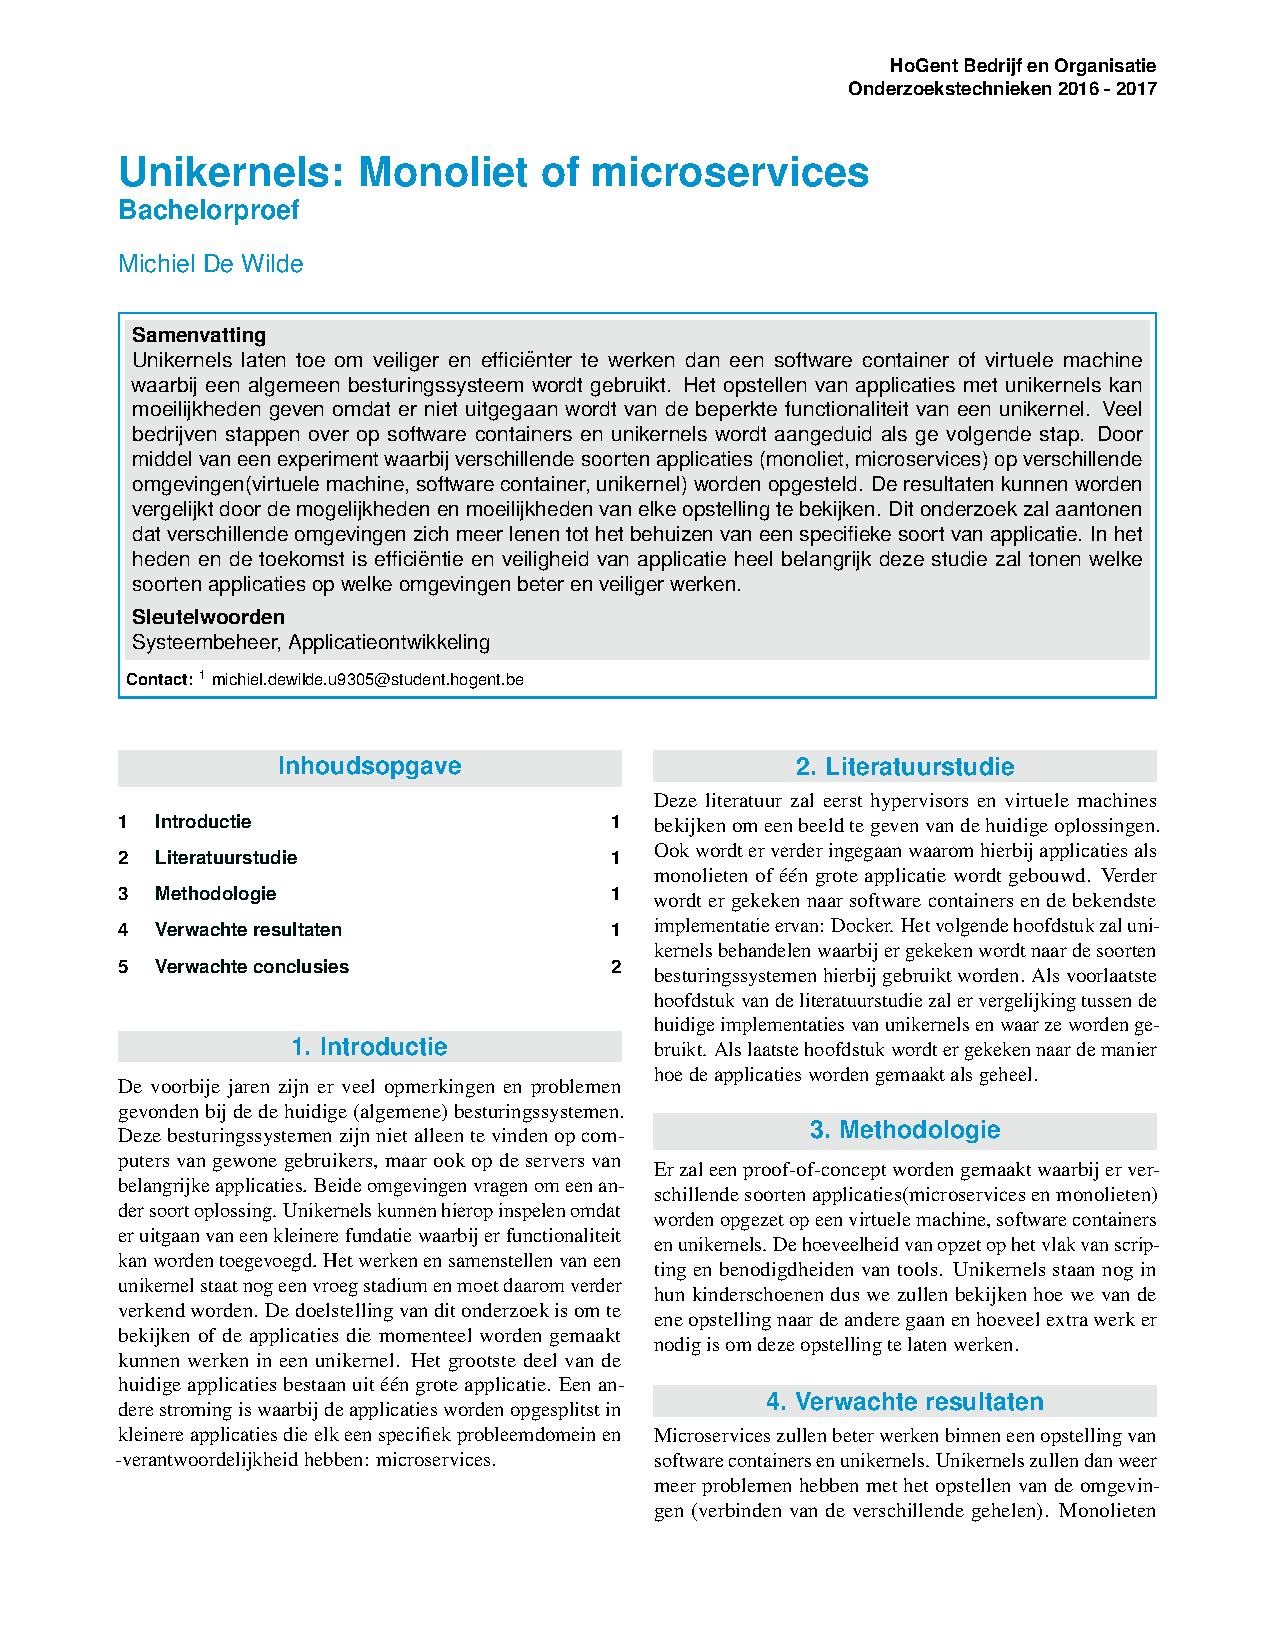
\includepdf[pages=-]{dewilde_michiel_voorstel}

%%---------- Back matter -------------------------------------------------

\printbibliography[title=Bibliografie]
\addcontentsline{toc}{chapter}{\textcolor{maincolor}{{Bibliografie}}}

\listoffigures
\listoftables

\end{document}
